%% Copyright (C) 2009 by Tobias Elze
%% Journal of Vision LaTeX template version 1.0
%% This document may be used freely for your own submissions.

\documentclass{jov}
\usepackage{graphicx} % needed for figures
\usepackage{subcaption}
\usepackage{hyperref}
\usepackage{amsmath}
\usepackage{bbm}
\usepackage{amssymb}
\usepackage{comment}

\DeclareMathOperator*{\argmin}{arg\,min}

\begin{document}

\title{Luminance constancy under fixed geometry}
\abstract{The light that reflects off an object surface and is captured by our eyes varies significantly with its context. But, the human visual system has the ability to stably perceive the object's color invariant of the context variations. The mechanism of this behaviorally significant invariance detection ability remains largely unknown. To understand the computational principles that lead to such invariant perception, we study the perception of object luminance under spectral variations in 3D scenes. Specifically, we study the effects of variations in reflectance and illumination spectra in a scene on the perceived luminance of an object. We have developed a software that generates naturalistic multispectral images of 3D scenes with precise control over the geometrical and spectral properties of the constituents that make a scene. We label these images with the luminance of a specific object in the scene. Next, we simulate the response of the retinal cones to these multispectral images using an accurate model of the early visual system. We then use supervised learning methods on these labeled cone response to identify the computations that lead to accurate luminance estimation. We show that if only either target, or background, or illumination spectra are allowed to vary, the standard luminance can be estimated through simple transformations of the cone responses. When all the spectra vary simultaneously, while it is not easy to recover the luminance through simple transformations, a decoding scheme that compares the light from the target and the surround, and properly adds the response of the L,M and S cones can recover the luminance within about 15\% RMSE.}

\author{Singh}{Vijay}
 {Computational Neuroscience Initiative}
 {and Department of Physics, University of Pennsylvania, PA, USA}
 {}{vsin@sas.upenn.edu}

\keywords{color constancy, luminance constancy, supervised learning}

\maketitle

\section{Introduction}
The perceived color of an object has important behavioral implications, since color helps us to identify objects and their properties \cite{Mollon89, Jacobs81}.
Perceived object color is not sensed directly, rather it is computed by the brain starting with the retinal image of the light reflected from an object to the eye.
The challenge of object color perception is that this reflected light depends not just on the object's surface reflectance, but also on extrinsic factors such as the illumination, the object's pose and the position of the observer (Fig.~\ref{fig:introSchematic}).
Thus, to produce a stable perceptual representation of an object's surface reflectance in the face of variation in these extrinsic factors, the brain must account for their influence on the reflected light.
The ability of a visual system to extract such a stable representation is called color constancy. Although human color constancy is by no means perfect, it is often very good \cite{FosterColorConstancy, BrainardColorConstancy}. 
In this paper, we consider the computational problem of color constancy, that is, how in principle could a visual system process the light reflected to the eyes to produce percepts well-correlated with object surface reflectance.

There is a considerable literature on computational color constancy. Seminal work considered a reduced scene model in which flat matte surfaces were illuminated by a single spatially diffuse illuminant and explored algorithms that could either recover a descriptor correlated with object surface reflectance (e.g. \citeNP{LandRetinex}) or produce explicit estimates of object surface reflectance and/or illuminant spectral power distribution (e.g., \citeNP{LandRetinex,Buchsbaum80,MaloneyWandell86}).
An important insight of this line of research was that, to account for variation in illumination, it was necessary to consider the light reflected from the entire scene. That is, although good constancy cannot be achieved in the face of illuminant variation if one considers only the light reflected from a single target object, when one considers the entire image it is possible to use the joint variation in light reflected from many objects to obtain (either implicitly or explicitly) an estimate of the illuminant common across the objects, and in turn to use this estimate to produce a stabilized representation of object color.
At the same time, this processing introduces an additional dependence.  Although the reflectance of the objects surrounding an object of interest has little direct effect on the light reflected from the object of interest, variation in the reflectance of the surrounding objects can have a large effect on the output of constancy algorithms that process the entire image \cite{BrainardWandellRetinex}.
Thus, a key aspect evaluating computational constancy algorithms is not only to ask about target object color stability with respect to variation in illumination, but also to ask about target object color stability with respect to the surface reflectance of other objects in the scene.
Subsequent computational constancy work sought to generalize both the image formation model to include richer geometric descriptions and to incorporate probabilistic descriptions of the statistics of naturally occurring scenes \cite{funt1988color, D'ZmuraConstancy3, barron2012color, D'ZmuraIversonSinger,BrainardFreeman}; LET'S SEE IF WE CAN FIND SOME RECENT REVIEWS).  None-the-less, it is not known how best to estimate stable object descriptors from images of the natural scenes we view in daily life.

% Figure 1: Introduction
\begin{figure}
\centering
\begin{subfigure}{0.4 \textwidth}
		\centering
        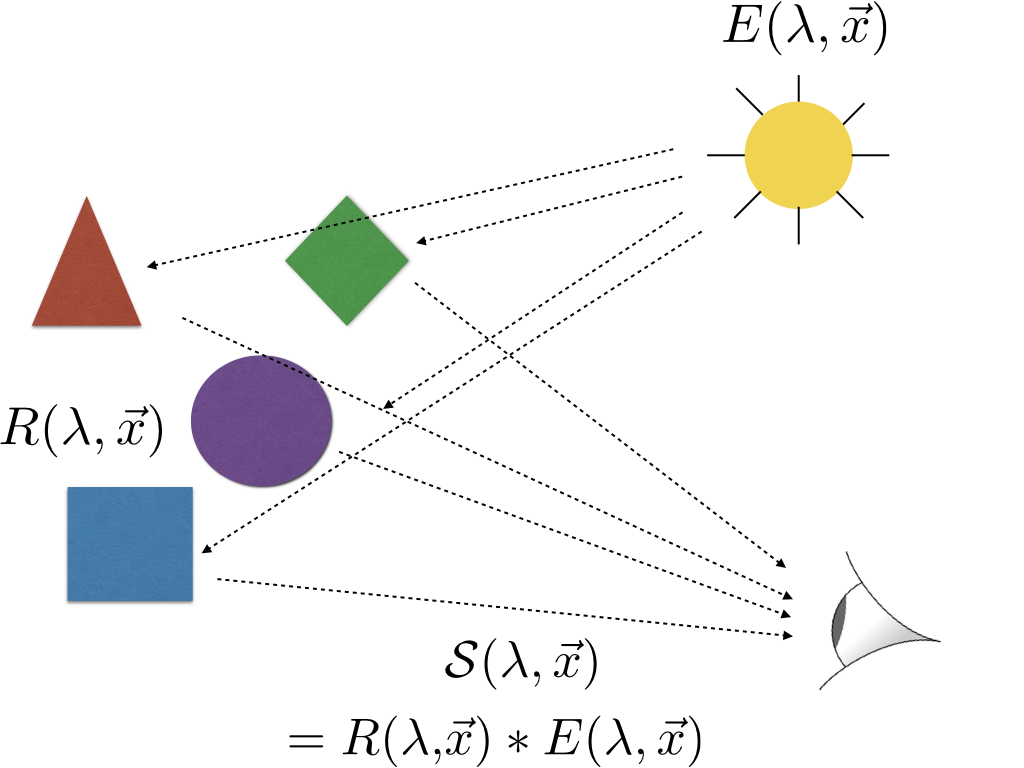
\includegraphics[width=\textwidth]{../Figures/Figure1/Figure1_a.png}
        \caption{}
        \label{fig:introSchematic}
    \end{subfigure}
    \begin{subfigure}{0.45 \textwidth}   
        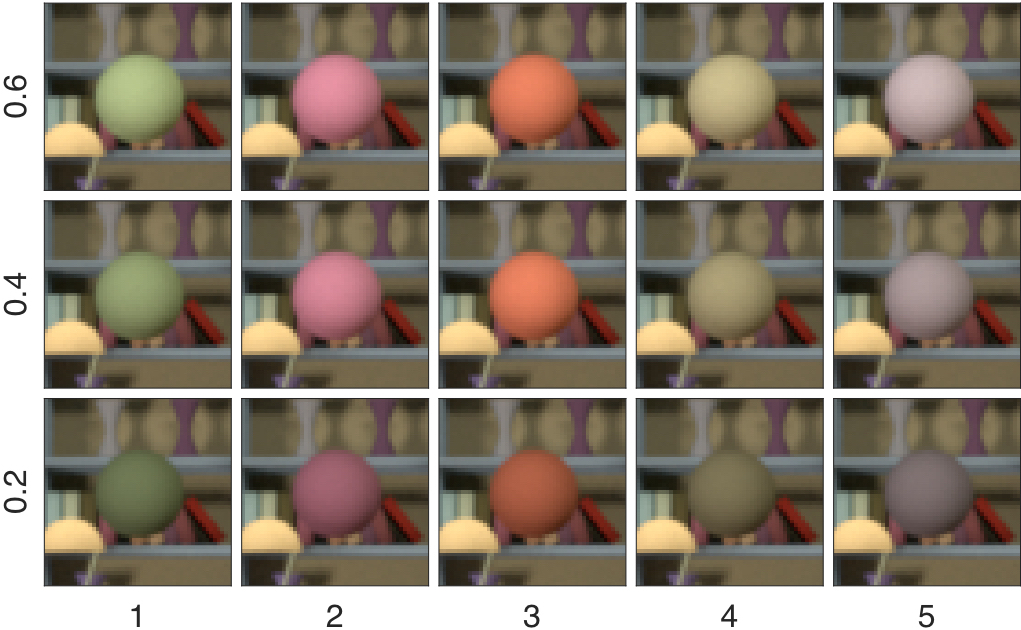
\includegraphics[width=\textwidth]{../Figures/Figure1/Figure1_b.jpeg}
        \caption{}
        \label{fig:introExampleFigure}
    \end{subfigure}
    \label{introFigure}
    \caption{(a) {\bf Color Constancy:} The light reflected from an object to our eyes depends both on the surface reflectance of the object, $R(\lambda,\vec{x})$, and the illumination spectrum of the light source, $E(\lambda,\vec{x})$. Additionally, it depends on geometric factors, such as the object's shape and pose, as well as the position of the observer. The human visual system is able to account for, at least partially, variations in the reflected light due to such extrinsic factors, and produce a percept of object color that is relatively stable with respect to such variations. Such invariant color perception is called color constancy. (b) {\bf Luminance Constancy Under Spectral Variations:} In this paper we consider the special case of luminance constancy. Fig.~\ref{fig:introExampleFigure} shows images of an object (the sphere in the center of each image) at three levels of object luminance (indicated on the left). Within each row, the surface reflectance of the spheres has the same luminance when illuminated by a standard reference illuminant, CIE D65. The three rows differ in this value, as can be seen by the fact that the luminance of the spheres generally decreases as we move down the columns. Within each row, the relative surface reflectance of the spheres varies, as can be seen by the variation in color appearance across the each row.  Within each column, this relative surface reflectance is held fixed. For illustration, we have kept the light source and the background objects fixed across the panels. See Fig.~\ref{fig:studiedCases} for images with such variations. In this paper, we seek to identify computations that accurately estimate object luminance across variations in relative surface reflectance, variations in illumination, and variation in the reflectance of other objects in the scene.}
 \end{figure}

The computational work reviewed above is based on formulating an explicit model of the image formation process and the statistical properties of natural images, and leveraging these formulations to obtain an appropriate ``inverse optics" algorithm.  An alternative approach, which has been less-well explored, is to use supervised machine learning techniques to develop mappings between input images and stable color descriptors.  Along these lines, Barron \cite{barron2015convolutional} recently developed a color balancing algorithm based on training a neural network to detect a uniform illuminant in an image by matching image templates in the chromaticity space. The use of supervised learning to understand human perceptual capabilities has enjoyed success in domains outside of color vision. Geisler and colleagues, for example, have developed a technique they refer to as accuracy maximization analysis (AMA, \citeNP{geisler2009optimal}), which learns linear filters whose output carries information that is optimized for particular perceptual tasks. This technique has provided computations that efficiently estimate speed \cite{burge2015optimal}, focus error \cite{burge2011optimal}, and disparity \cite{burge2014optimal} 
from image patches taken from natural scenes, and that in addition provide excellent models of human's ability to make corresponding estimates from the same stimuli.  In this paper, we apply AMA, as well as comparison supervised learning algorithms to a special case of the color constancy problem (luminance constancy) and evaluate how well it performs for naturalistic image input. 

A difficulty in using machine learning approaches for color constancy is that these approaches require large training sets with images of scenes containing objects with known surface reflectances illuminated with known illuminations.  Such data sets are not readily available. Although there are several databases of calibrated color natural images, these do not generally provide the corresponding information about surface and illuminant ground truth \cite{ChakrabartiHyperspectral,NascimentoFoster2016,ParragaHyperspectralData,TkacikUpennHypersepctralData,skauli2013collection,olmos2004biologically}. 
Generating databases with both the images and the ground truth scene information is not trivial. One approach has been to acquire images where objects of known reflectance have been inserted into the scene, and to use the image of these reference objects to provide an estimate of the illumination impinging at various scene locations \cite{NascimentoFoster2016}.  This is somewhat painstaking, however, and in any case provides information about the illumination only at a small number of selected locations, so that generalizing across the image requires strong assumptions. Some progress is being made on characterizing how illumination varies over space in natural scenes \cite{mury2007spatial}, which in the longer run may guide how information from reference objects can be used to provide reasonable estimates.  Another approach is to acquire images of posed scenes, where the surface reflectances of objects are measured individually for many of the objects in the scene \cite{funt1988color,ciurea2003large, davidPennHyperspectral}. 
% REMOVE NO DATE (n.d.) FROM THE CITATION
These data sets have been useful for evaluating computational color constancy algorithms, but the use of posed scenes does not scale well for use with supervised learning methods which needs large training sets. 
 
% Figure 2: Cases Studied
\begin{figure}
\centering
	\begin{subfigure}[b]{0.33 \textwidth}
		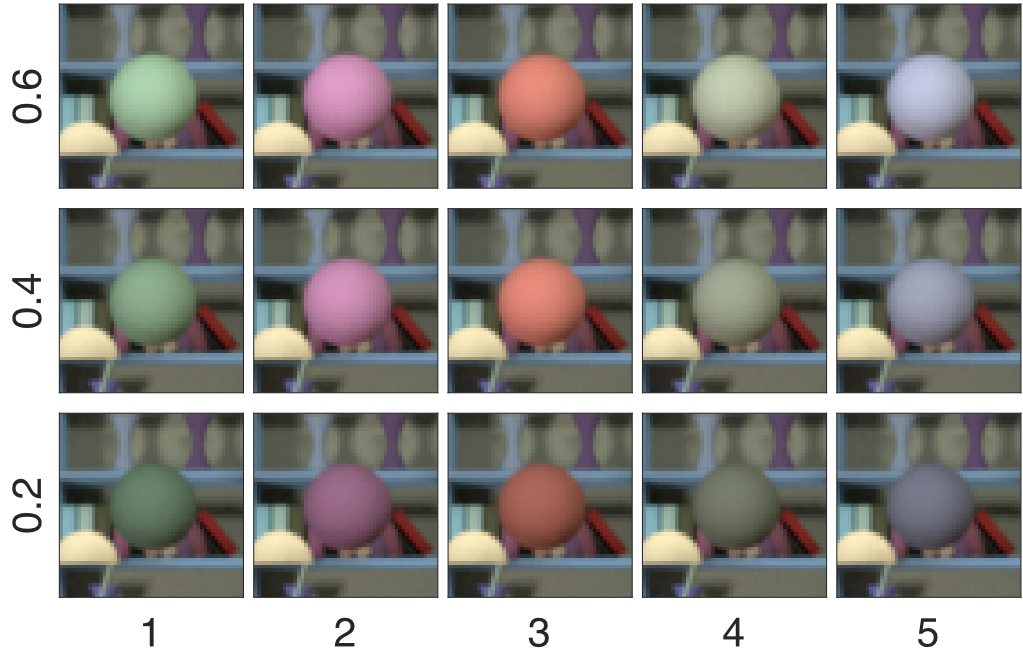
\includegraphics[width=\textwidth]{../Figures/Figure2/Figure2_a.jpeg}
		\caption{Case 2}
 		\label{fig:backgroundVarying}
	\end{subfigure}
	\begin{subfigure}[b]{0.33 \textwidth}
        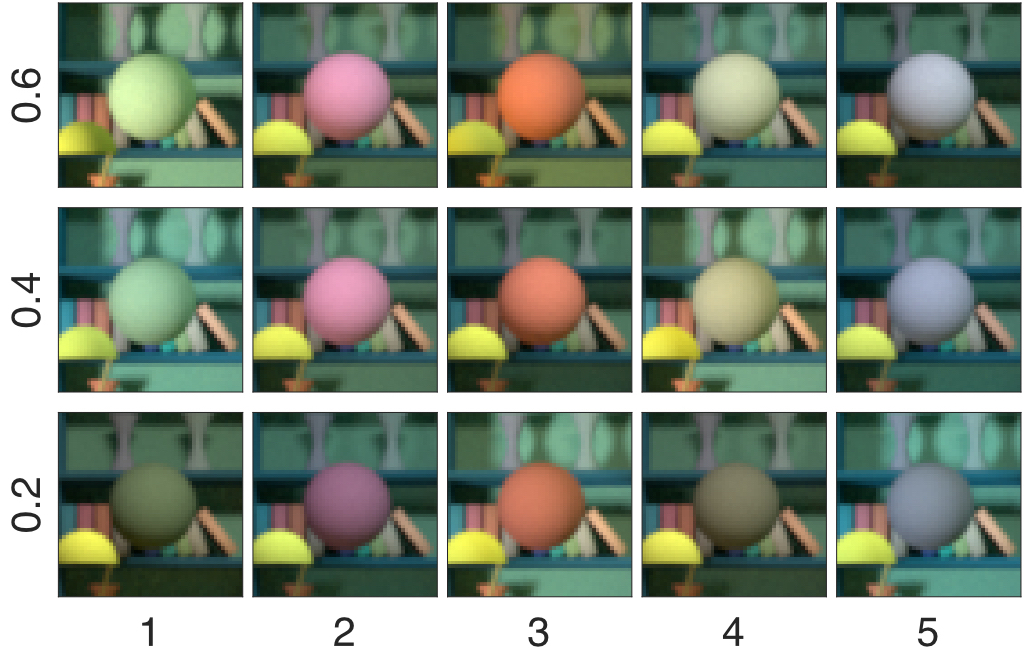
\includegraphics[width=\textwidth]{../Figures/Figure2/Figure2_b.jpeg}
        \caption{Case 3}
        \label{fig:targetIlluminantVarying}
    \end{subfigure}
	\begin{subfigure}[b]{0.33 \textwidth}
        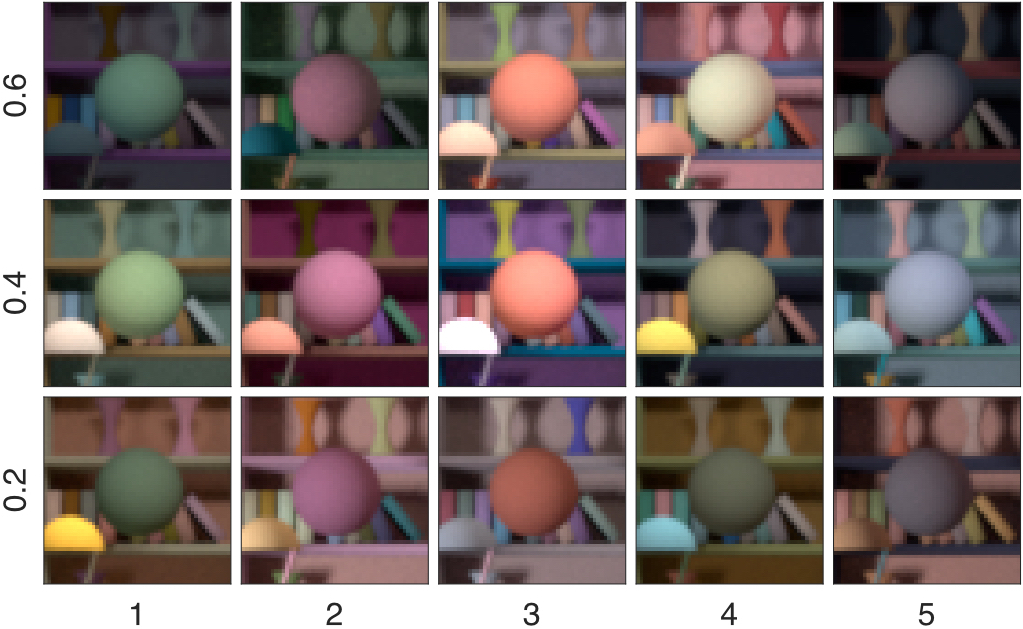
\includegraphics[width=\textwidth]{../Figures/Figure2/Figure2_c.jpeg}
        \caption{Case 4}
        \label{fig:allSpectraVarying}
    \end{subfigure}    
    \caption{{\bf Types of spectral variations studied in this work:} sRGB rendition of multispectral images similar to ones studied in our work. The numbers on the left indicate the standard luminance level of the target object. 5 images are shown at each luminance level. We studied four types of spectral variations. Case 1: target object relative surface reflectance spectrum variable, light source spectra fixed, background object spectra fixed, (Fig.~\ref{fig:introExampleFigure}). (a) Case 2: target object relative surface reflectance spectrum variable, light source spectra fixed, background object spectra variable, (b) Case 3: target object relative surface reflectance spectrum variable, light source spectra variable, background object spectra fixed, (c) Case 4: target object relative surface reflectance spectrum variable, light source spectra variable, background object spectra variable. As in \ref{fig:introExampleFigure}, the spheres in each row of each panel have the same surface luminance, while the spheres in each column of each panel have the same relative surface reflectance.  Moreover, across the four panels (Fig.~\ref{fig:introExampleFigure} \& Fig.~\ref{fig:studiedCases}), spheres in corresponding locations have the same surface reflectance. In all four panels, the overall lights source spectra scale factors (see \nameref{Methods}) were drawn from a uniform distribution on the range [0.5, 1.5]. The sRGB values for all three panels were normalized using a common scale factor prior to gamma correction.} 
\label{fig:studiedCases}
\end{figure}

Because of the difficulty in obtaining large labelled data sets of natural images for use in developing and evaluating computational color constancy algorithms, in this paper we adopt the approach of using high-quality computer graphics to render images of what we refer to as {\em virtual natural scenes}. Here, in addition to employing computer graphics to render the light reaching the eye from specified scenes, we also model the initial steps of the human visual system, so that our supervised learning methods are applied not to image pixels but rather to modeled responses of the foveal cone photoreceptor mosaic. We describe this approach in detail below. The key advantage of this approach is that we can produce large numbers of naturalistic images and the corresponding cone mosaic responses where all of the underlying scene properties are well-specified. This allows us to explore and evaluate computational color constancy with rich stimuli, while retaining the ability to precisely control and manipulate the intrinsic properties of the objects and illuminants that comprise the scene. This general approach has been adopted by other labs for the study of computational estimation of optical flow \cite{baker2011database} and is becoming increasingly popular \cite{kovacs17shading},
% Autonmous vehicle work - ask BAW
as well as for the generation of stimuli for the study of human perception (e.g., \citeNP{boyaci2003effect, todd1983perception, arend1986Simultaneous, johnston1993integration}). 
Of course, success within the domain of graphics images does not guarantee smooth generalization to real natural images, a point we return to in the \nameref{Discussion}.

In this initial work, we do not tackle the full problem of color constancy.  Rather, as a point of departure, we consider the computational problem of estimating a single attribute of object surface reflectance, which we refer to as surface luminance.  We compute object luminance from an object's surface reflectance function as follows.  We compute the light that would be reflected to the eye from a flat matte object with that surface reflectance, when the object is diffusely illuminated by the standard CIE daylight spectrum D65 \cite{CIE86}.  We then compute the luminance of this reflected light, using the CIE 1931 photopic luminosity function \cite{CIE86}, and divide this by the luminance of a perfectly reflecting diffuser (surface reflectance of one at all wavelengths) when that is computed in the same way. This procedure allows us to assign to any surface reflectance a single surface luminance value.  Because the perceived luminance of an object is approximately (but by no means exactly, see \citeNP{wyszecki1986color}) correlated with surface luminance across a range of viewing conditions, we refer to the computational problem we study as that of {\em luminance constancy}.
This is a generalization of the way this term is often used, where it refers more specifically to the stability of perceived luminance across images of scenes where all objects and illuminants are achromatic \cite{gilchrist2006seeing}.
Here, we aim to estimate surface luminance, but do so for images where both the luminance and the chromaticity of the surfaces and illuminants varies (see  Fig.~\ref{fig:introExampleFigure}). A particularly important feature of our treatment is that we consider scene variations where not only the spectrum of the illumination varies, but also the surface reflectance of objects in the scene other than the object whose surface luminance is being estimated. 

Even within the special case of luminance constancy, there are many scene manipulations that could be considered. The set of manipulations we focus on here are illustrated by Fig.~\ref{fig:introExampleFigure} and the three panels of Fig.~\ref{fig:studiedCases}. These cases are: 1. variation in target object spectrum with fixed light source and background objects spectra (Fig.~\ref{fig:introExampleFigure}), 2. variation in target object spectrum and background objects spectra, with fixed light source  (Fig.~\ref{fig:backgroundVarying}), 3. variations in both the target object spectrum and the light source spectra, with fixed background object spectra (Fig.~\ref{fig:targetIlluminantVarying}), and 3. variations in all three types of spectra (target object, light source, and background objects) (Fig.~\ref{fig:allSpectraVarying}). Across real scenes, there will also be variations in the shape of the target object, its pose, eye position, etc. (see \nameref{Methods}). In this paper, we focus on the problem of luminance constancy within scene ensembles where these geometric factors are held fixed.

We show that for cases that have spectral variation only either in target object surface reflectance or background object surface reflectance or the power spectrum of the light sources, luminance can be estimated by simple transformations of the cone responses. For variations only in target object reflectance spectra (case 1) or just the target and background objects reflectance spectra (case 2), object luminance can be recovered directly from the light reflected off the target object. For case 3, where both the target object reflectance and light source spectra vary, object luminance can be recovered from the contrast between the target and the background. When all the spectral features in the scene are allowed to change (case 4), the standard luminance can not be recovered simply from the cone response or the contrast. We have used AMA with a Bayesian estimator to estimate standard luminance of the target object. Using this method, we can recover the luminance of the target object with $\sim 15\%$ relative root mean square error.  Our analysis shows that the optimal receptive fields for estimating the luminance of the target object show a center surround structure, supporting a comparison between the light coming from the target object and its surround. Additionally, luminance estimation involves a weighted sum of the L, M and S cone responses where the receptive fields give more weight to the L and M cone responses compared to S cone responses. Comparing the performance of the RFs learnt using  one case on the cone response of other cases shows that the receptive field of the complex cases perform well on images of simpler cases. We discuss the implications of such receptive fields on luminance constancy. 

The rest of this paper is organized as follows. In the \nameref{Methods} section, we describe in detail the process to generate naturalistic labeled images (\nameref{method:VirtualWorld}) using our software pipeline {\rm Virtual world color constancy}, the process to simulate the response of retinal cone photoreceptors to these images using a standard model of the early visual system (\nameref{method:Isetbio}) and the supervised learning method (AMA) used in our analysis (\nameref{method:SupervisedLearning}). In the \nameref{Results} section, we show the estimates and performance of the supervised methods for the four cases mentioned above. We conclude the paper with the implication of our results in the \nameref{Discussion} section.  

\section*{Methods} \label{Methods}
\subsection{Overview}
There are four key parts to our methods.  The first is how we generate a labelled set of training data for our supervised learning algorithms.  The second is how we model the transformations applied by the early visual system to generate modeled responses of the cone photoreceptor mosaic.  The third is the details of the supervised learning method (AMA) that we apply to the labelled training data.  And the fourth is how we evaluate the performance of the algorithm.  We describe each of these in the sections below.

\subsection{Labelled image database} \label{method:VirtualWorld}

% Figure 3
\begin{figure}[t]
\centering
\begin{subfigure}[b]{0.22 \textwidth}
        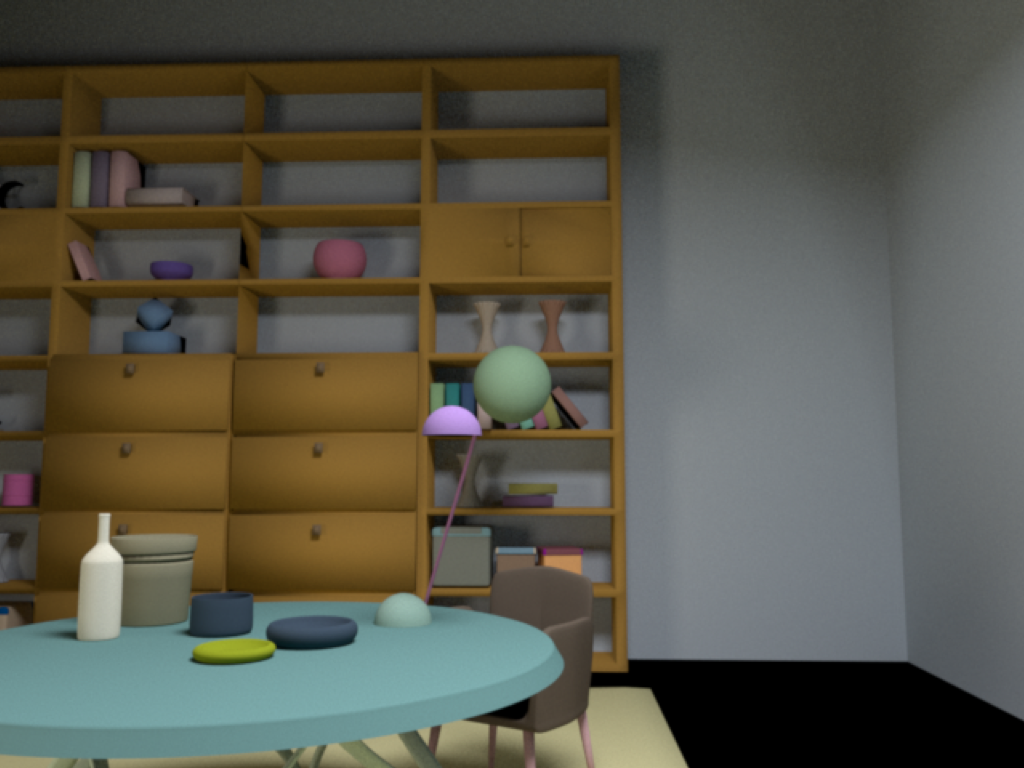
\includegraphics[width=\textwidth]{../Figures/Figure3/Figure3_a.png}
        \caption{Library }
        \label{fig:baseSceneLibrary}
    \end{subfigure}
    ~
    \begin{subfigure}[b]{0.22 \textwidth}
        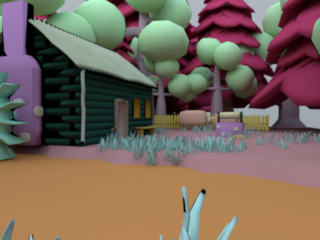
\includegraphics[width=\textwidth]{../Figures/Figure3/Figure3_b.png}
        \caption{Mill}
        \label{fig:baseSceneMill}
    \end{subfigure}    
    ~
    \begin{subfigure}[b]{0.22 \textwidth}
        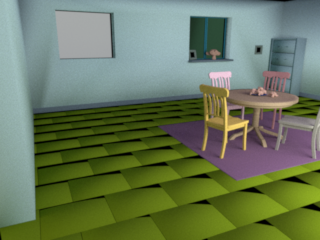
\includegraphics[width=\textwidth]{../Figures/Figure3/Figure3_c.png}
        \caption{Table-Chairs}
        \label{fig:baseSceneTableChairs}
    \end{subfigure}
    
    \begin{subfigure}[b]{0.22 \textwidth}
        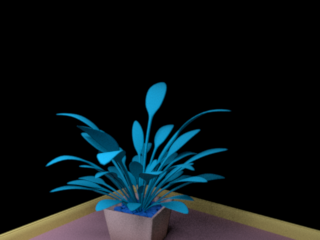
\includegraphics[width=\textwidth]{../Figures/Figure3/Figure3_d.png}
        \caption{Indoor-plant}
        \label{fig:baseSceneIndoorPlant}
    \end{subfigure}    
    ~
    \begin{subfigure}[b]{0.22 \textwidth}
        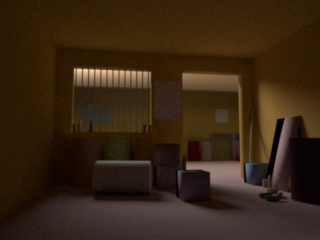
\includegraphics[width=\textwidth]{../Figures/Figure3/Figure3_e.png}
        \caption{Warehouse}
        \label{fig:baseSceneWarehouse}
    \end{subfigure}
    ~
    \begin{subfigure}[b]{0.22 \textwidth}
        
\includegraphics[width=\textwidth]{../Figures/Figure3/Figure3_f.png}
        \caption{Checkerboard}
        \label{fig:baseSceneCheckerBoard}
    \end{subfigure}
    \caption{{\bf Example of base scenes form the VWCC library.} Each panel shows a rendering of one tamed base scene without additional objects inserted.  The reflectance spectra of the distinct surfaces in each scene has been assigned randomly (see below) using the VWCC software.  The light source spectra were also assigned randomly to the default and inserted light source.}\label{fig:baseScenes}
\end{figure}

\subsubsection{Virtual naturalistic scenes}
The light that reflects off an object and reaches our eyes depends on many factors. These factors include: the surface reflectance of the object, the surface reflectance, texture, material and geometry of the objects in its surround, the spectrum of the sources of light illuminating the object, and the position of the observer. In natural scenes, these spectral and geometrical factors vary considerably. To study the effect of these factors on color perception, we need a system that can generate natural scenes with precise control over all such factors. We need a system that can produce natural scenes at a fixed perceived color of a target object, while having a representative, but precisely quantified, sampling of the variations in the scene. Under natural conditions it is difficult to control and quantify every such parameter in a scene. Thus generating such a dataset, with a representative sampling of natural variations, is considerably time and labor intensive.

To overcome this  challenge, we have developed an image rendering software pipeline that allows us to specify a virtual, but naturalistic, statistical model of visual scenes with parametric control over factors in natural scenes. The software uses a physically-based image rendering system that accurately accounts for the interactions of light with matter in 3D scenes. It then renders a multispectral 2D image of each modeled visual scene. Wherever possible, we have incorporated statistical models of the variation of specific scene parameters based on observed data in natural scenes. In addition, our software simulates the responses of retinal cones to the rendered multispectral images using a realistic model of the early human visual system. Below we provide the details of the software and the choices made to generate ensembles of scenes with corresponding images. Our software, which is written in MATLAB, is freely available through a public respository: \href{https://github.com/BrainardLab/VirtualWorldColorConstancy}{Virtual World Color Constancy}. It builds on several other open source projects, including \href{http://rendertoolbox.org}{RenderToolbox4} \cite{heasly2014rendertoolbox3}, \href{http://isetbio.org}{Isetbio} and \href{https://www.mitsuba-renderer.org}{Mitsuba} \cite{jakob2015mitsuba}. Below we refer to the software pipeline as VWCC (for Virtual World Color Constancy).

% Figure 4
\begin{figure}
\centering
\begin{subfigure}[b]{0.14 \textwidth}
        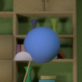
\includegraphics[width=\textwidth]{../Figures/Figure4/Figure4_a.png}
        \caption{Big-ball}
        \label{fig:libraryWithBigBall}
    \end{subfigure}
    ~ 
\begin{subfigure}[b]{0.14 \textwidth}
        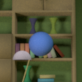
\includegraphics[width=\textwidth]{../Figures/Figure4/Figure4_b.png}
        \caption{Small-ball}
        \label{fig:libraryWithSmallBall}
    \end{subfigure}
    ~ 
    \begin{subfigure}[b]{0.14 \textwidth}
        
\includegraphics[width=\textwidth]{../Figures/Figure4/Figure4_c.png}
        \caption{Barrel}
        \label{fig:libraryWithBarrel}
    \end{subfigure}
    \begin{subfigure}[b]{0.14 \textwidth}
        
\includegraphics[width=\textwidth]{../Figures/Figure4/Figure4_d.png}
        \caption{Xylophone}
        \label{fig:libraryWithXylophone}
    \end{subfigure}
    ~
	\begin{subfigure}[b]{0.14 \textwidth}
        
\includegraphics[width=\textwidth]{../Figures/Figure4/Figure4_e.png}
        \caption{Ring toy}
        \label{fig:libraryWithRingToy}
    \end{subfigure}
        ~
    	\begin{subfigure}[b]{0.14 \textwidth}
        
\includegraphics[width=\textwidth]{../Figures/Figure4/Figure4_f.png}
        \caption{Bottle}
        \label{fig:libraryWithChampagneBottle}
    \end{subfigure}
\caption{{\bf Library base scene with inserted objects.} The VWCC software was used to insert different objects into the library base scene, with each panel showing a different object. The objects were inserted at a location in the image and then the camera was pointed at the object, so that the object's image is at the center of the rendered image.  In the figure panels, the full rendered image is cropped so that the inserted object is more visually salient. We use this capability of our software pipeline to insert target objects into scenes.}\label{fig:libraryWithTarget}
\end{figure}

The process of generating an individual virtual scene begins with the selection of a \textit{base scene} (Fig.~\ref{fig:baseScenes}). The base scene is a 3D model that defines a rendering space.  It typically includes the specification of a number of 3D objects and light sources, and is annotated with meta-data that may be used to guide the placement of additional objects and light sources, as well as the specification of camera position. VWCC includes a library of base scenes obtained from materials made available on the Internet under various Creative Commons licenses. We have found that there is sufficient variation in how nominally-standard graphics interchange file formats are used in practice that each base scene obtained from the Internet (which we refer to as \textit{wild scenes}) requires a certain amount of hand editing before it renders properly. We refer to this process, along with adding meta-data about the scene, as \textit{taming} a wild scene. Tame base scenes may also be created {\it de novo} using a 3D modeling software (e.g., \href{https://www.blender.org/}{Blender}).  The overall spatial scale of the base scene may be adjusted under programmatic control or chosen randomly, adding to the available statistical richness. If one chooses to draw entries from the base scene library at random for each virtual scene, the base scene library then provides a simple statistical model of the gross layout of natural scenes. As time progresses, we plan to tame more wild scenes so as to increase the number of entries in the base scene library. Currently the library contains 6 base scenes: Library (Fig.~\ref{fig:baseSceneLibrary}), Mill (Fig.~\ref{fig:baseSceneMill}), Table-Chairs (Fig.~\ref{fig:baseSceneTableChairs}), Indoor plant (Fig.~\ref{fig:baseSceneIndoorPlant}), Checkerboard (Fig.~\ref{fig:baseSceneWarehouse}) and Warehouse (Fig.~\ref{fig:baseSceneCheckerBoard}).

VWCC provides an option for inserting 3D objects and lights sources into the base scene. Fig.~\ref{fig:libraryWithTarget} shows examples of objects inserted into the library base scene. The object shapes may be selected from a VWCC library that, similar to the VWCC library of base scenes, has been tamed from object descriptions made available on the Internet. The light sources may be chosen as point lights, area lights, or as shapes selected from the object library. The position (Fig.~\ref{fig:targetPositionVariation}), size and orientation (Fig.~\ref{fig:targetSizeOrientation})of the inserted objects and lights may be specified programatically or chosen randomly under constraints provided by the base scene meta-data. Thus, along with distributions that characterize parameters such as the number, size, shape and orientation of the inserted objects and light sources, we have a simple statistical model of the object and light source geometry of natural scenes. 

% Figure5
\begin{figure}
\centering
	\begin{subfigure}[b]{0.18 \textwidth}
    \centering
        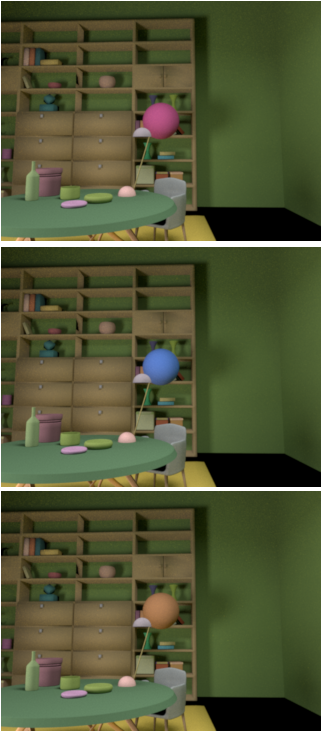
\includegraphics[width=\textwidth]{../Figures/Figure5/Figure5_a.png}
        \caption{Target spectra}
        \label{fig:targetVariation}
    \end{subfigure}
    ~
    \begin{subfigure}[b]{0.18 \textwidth}
    \centering
        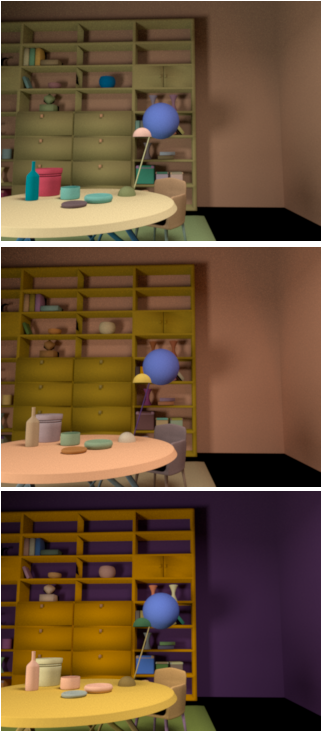
\includegraphics[width=\textwidth]{../Figures/Figure5/Figure5_b.png}
        \caption{Background spectra}
        \label{fig:backGroundVariation}
    \end{subfigure}
    ~
    \begin{subfigure}[b]{0.18 \textwidth}
    \centering
        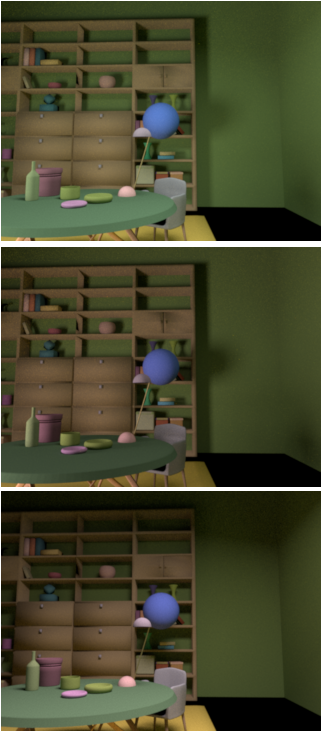
\includegraphics[width=\textwidth]{../Figures/Figure5/Figure5_c.png}
        \caption{Illumination spectra}
        \label{fig:illuminationVariation}
    \end{subfigure}
    ~
	\begin{subfigure}[b]{0.18 \textwidth}
    \centering
        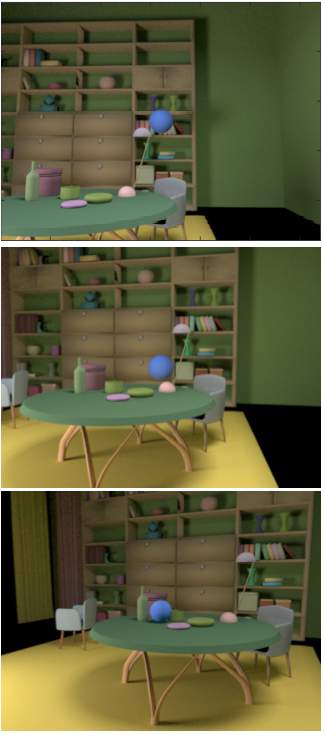
\includegraphics[width=\textwidth]{../Figures/Figure5/Figure5_d.png}
        \caption{Target position}
        \label{fig:targetPositionVariation}
    \end{subfigure}
    ~
	\begin{subfigure}[b]{0.18 \textwidth}
    \centering
        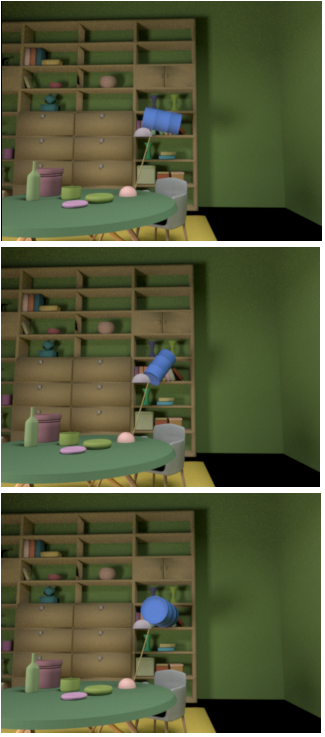
\includegraphics[width=\textwidth]{../Figures/Figure5/Figure5_e.png}
        \caption{Target Size/Orientation}
        \label{fig:targetSizeOrientation}
    \end{subfigure}
    ~
    \caption{{\bf Transformations of the scene.} The possible transformations of the properties of a scene can broadly be classified into two groups: Spectral (a-c) and Geometrical (d-e). VWCC provides control over such transformation as illustrated by the columns. (a) The target object surface reflectance varies across the three panels of the column. (b) The surface reflectance of the background objects varies across the three panels. In each panel, the reflectances were assigned randomly. (c) The power spectrum of the light sources were assigned randomly in the three panels. (d) The three panels in the column have the target object at three different positions. The camera points to the center of the pixel. }\label{fig:VWCCTransformations}
\end{figure}

Once a base scene has been chosen and objects and light sources inserted, we assign spectral surface reflectance, texture, and material property to each object surface in the scene. We also assign an illuminant spectral power distribution to each light source in the scene. Objects in the VWCC library may contain more than one distinct surface, each of which may be assigned a different surface reflectance. As with object position, these may be specified programatically. In the present work, we use simple choices for texture (all surfaces spatially uniform) and material property (all surfaces matte) and focus on variation in surface spectral reflectance. 

In the present work, we insert one target object and one additional light source into a fixed base scene, and vary reflectance and illuminant spectra. We then insert a camera for rendering at a user specified position and point this camera at the target object. We ensure that a 9 pixel by 9 pixel region at the center of the image corresponds to light reflected from the target object, which amounts to verifying that the target object at its inserted position was not occluded by other objects in the line of sight from camera. For each rendered scene, we specify the surface reflectance of the target object, which allows us to control both its surface luminance as well as its relative surface reflectance. The specified surface luminance provides the requisite label for the scene and resultant cone mosaic responses.

We render scenes using the \href{https://www.mitsuba-renderer.org}{Mitsuba} \cite{jakob2015mitsuba} rendering package, driven by our \href{http://rendertoolbox.org}{RenderToolbox4} \cite{heasly2014rendertoolbox3} rendering pipeline.

For the images used for the primary results reported in this paper, we used the ``{\it Library}'' base scene from the VWCC  and the ``{\it Big Ball}'' object as the target object. We also inserted a spherical light source with the same ``{\it Big Ball}'' shape. The position, and size of the inserted object, light source and the camera were held fixed for all the images analyzed in this work, i.e., the scene geometry did not vary. Next, we assigned illumination and surface reflectance spectra to the lights and objects in the scene. The spectral manipulations for the various cases studied in this work have been described in the main text (Fig.~\ref{fig:introExampleFigure} \& Fig.~\ref{fig:studiedCases}). 2D multispectral images were rendered at 31 wavelengths from $400$nm to $700$nm spaced $10$nm apart at an image size $320\times 240$ pixel. A $51 \times 51$ pixel patch of the multispectral image was cropped around the target object and cone responses were calculated to these cropped images. 

\subsubsection{Illumination Spectra}
% Figure 6
\begin{figure}
\centering
	\begin{subfigure}[b]{0.3 \textwidth}
    \centering
        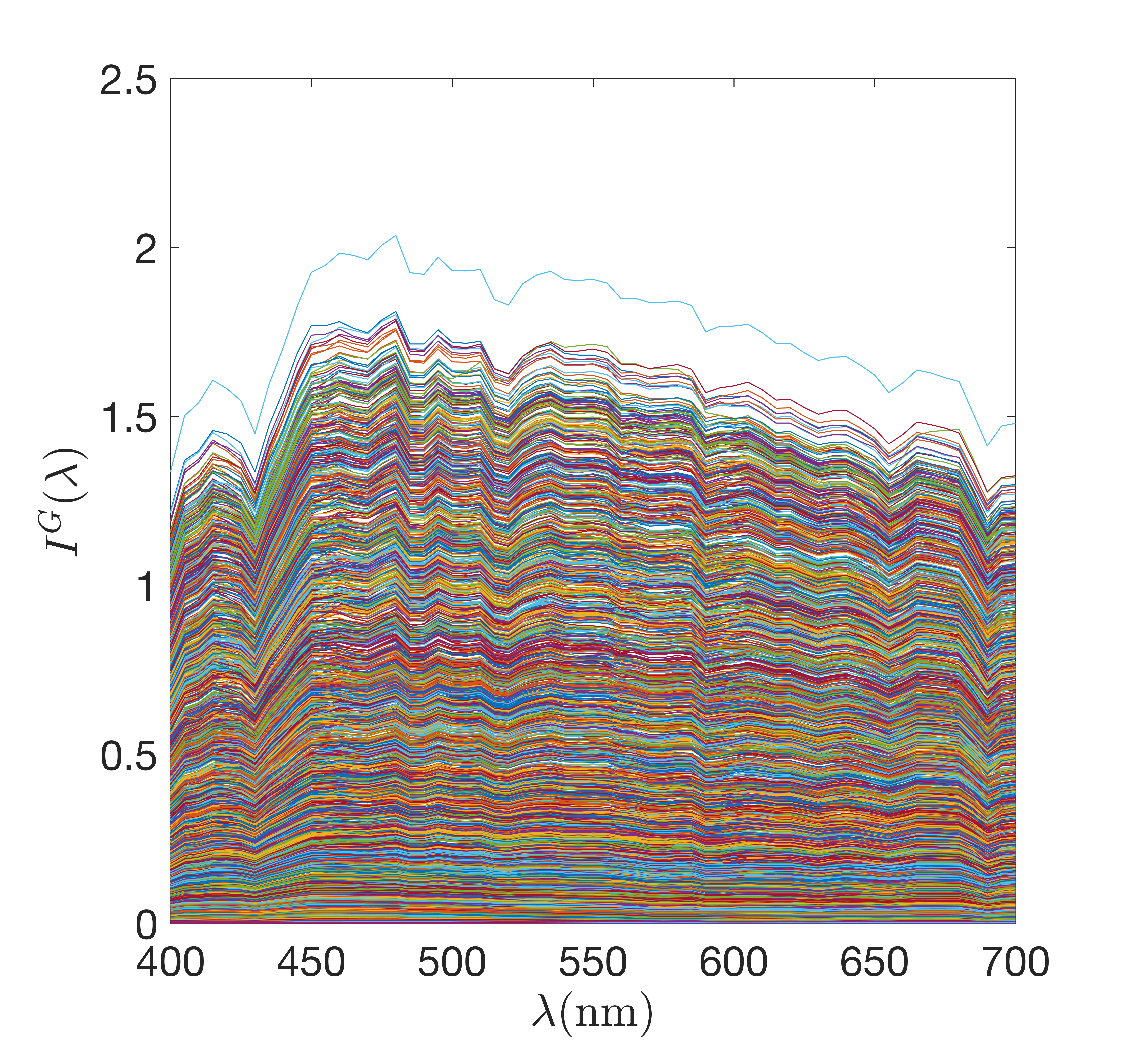
\includegraphics[width=\textwidth]{../Figures/Figure6/Figure6_a.pdf}
        \caption{Granada natural daylight dataset}
        \label{fig:granadaSpectra}
    \end{subfigure}
    \begin{subfigure}[b]{0.3\textwidth}
    \centering
        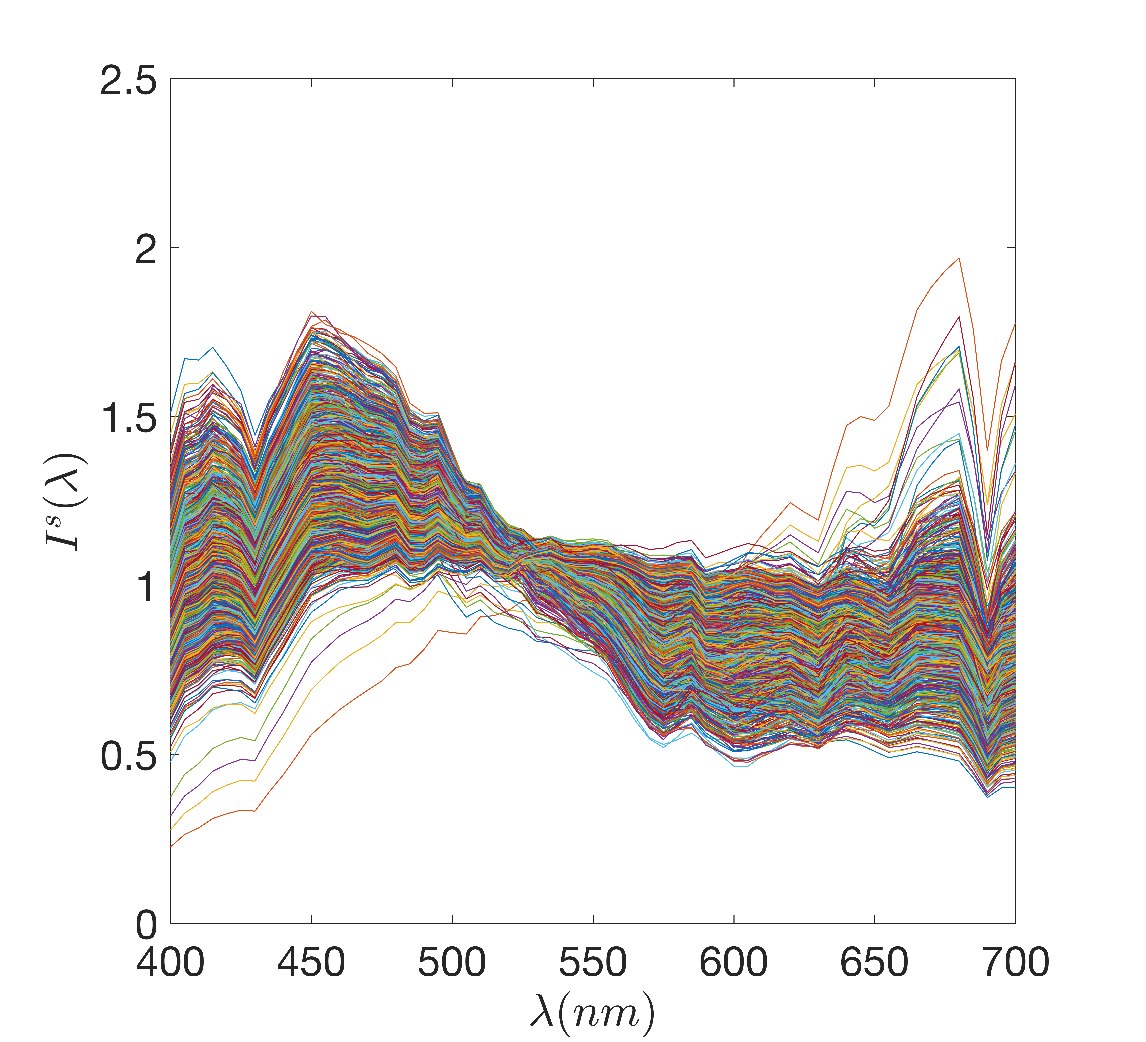
\includegraphics[width=\textwidth]{../Figures/Figure6/Figure6_b.pdf}
        \caption{Rescaled Granada dataset}
        \label{fig:rescaledGranada}
    \end{subfigure}
    \begin{subfigure}[b]{0.3 \textwidth}
    \centering
        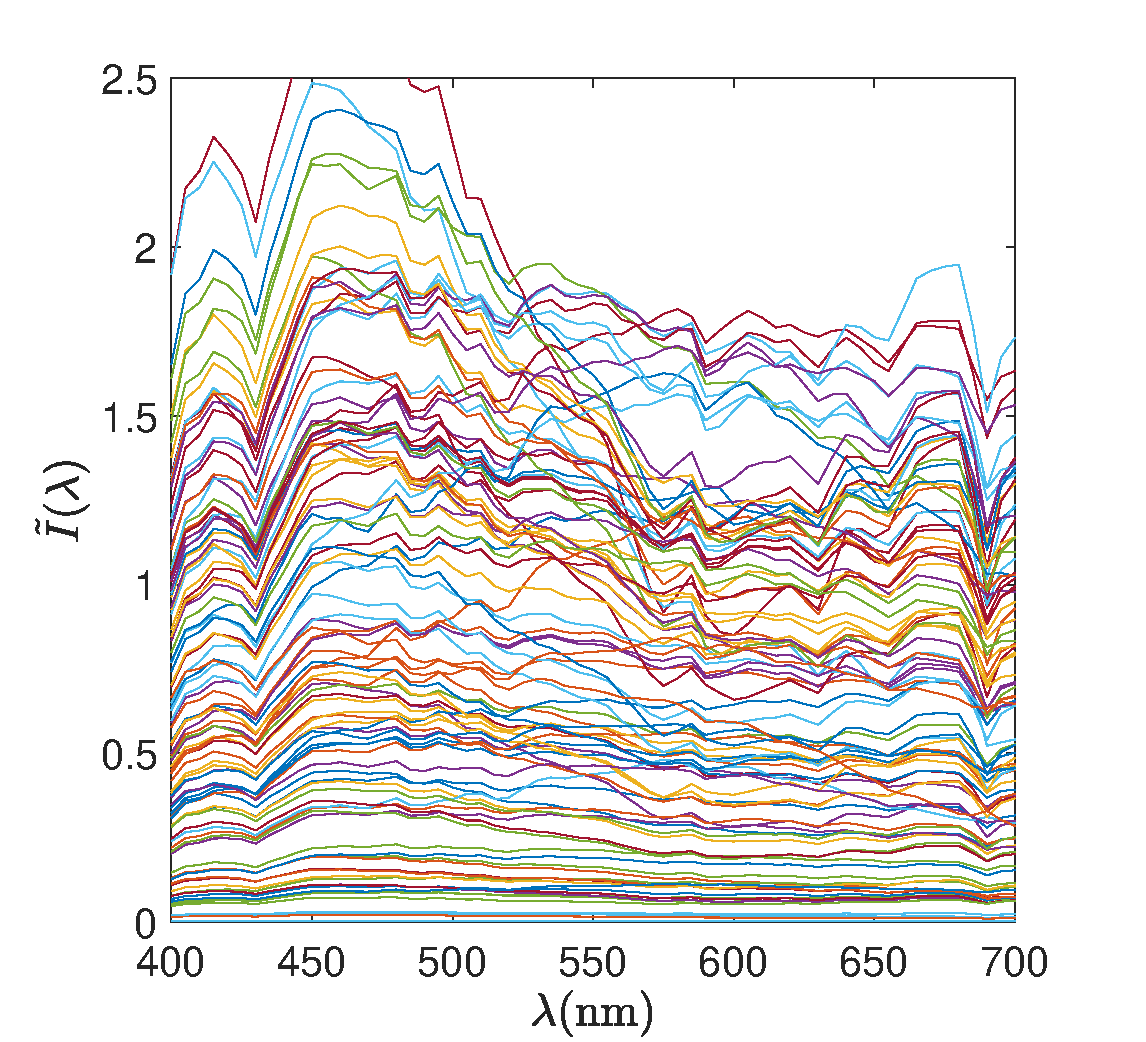
\includegraphics[width=\textwidth]{../Figures/Figure6/Figure6_c.pdf}
        \caption{Randomly generated samples}
        \label{fig:randomIlluminant}
    \end{subfigure}

	\begin{subfigure}[b]{0.3 \textwidth}
    \centering
        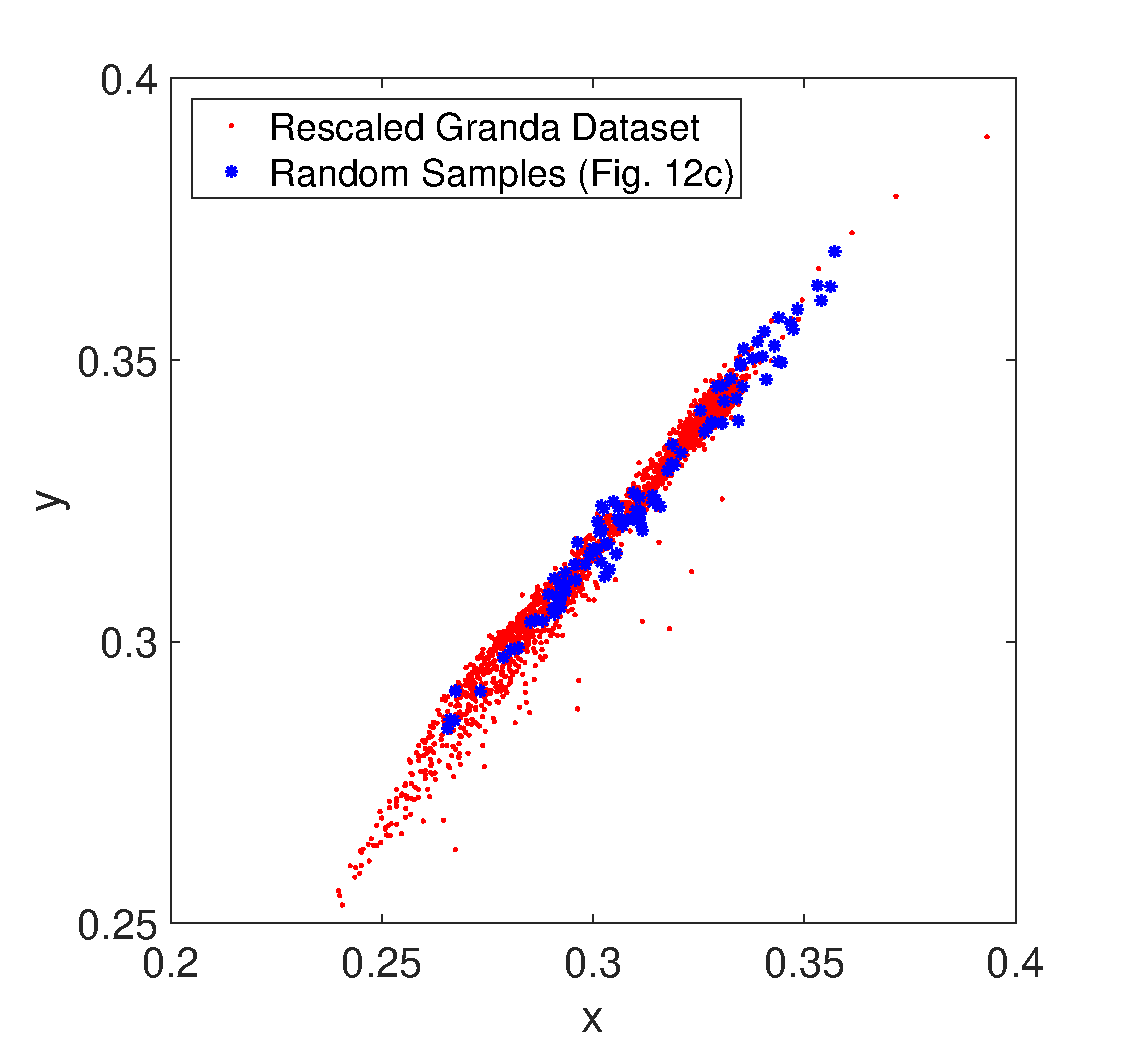
\includegraphics[width=\textwidth]{../Figures/Figure6/Figure6_d.pdf}
        \caption{Normalized PCA eigenvalues}
        \label{fig:granadaEV}
    \end{subfigure}
	\begin{subfigure}[b]{0.3 \textwidth}
    \centering
        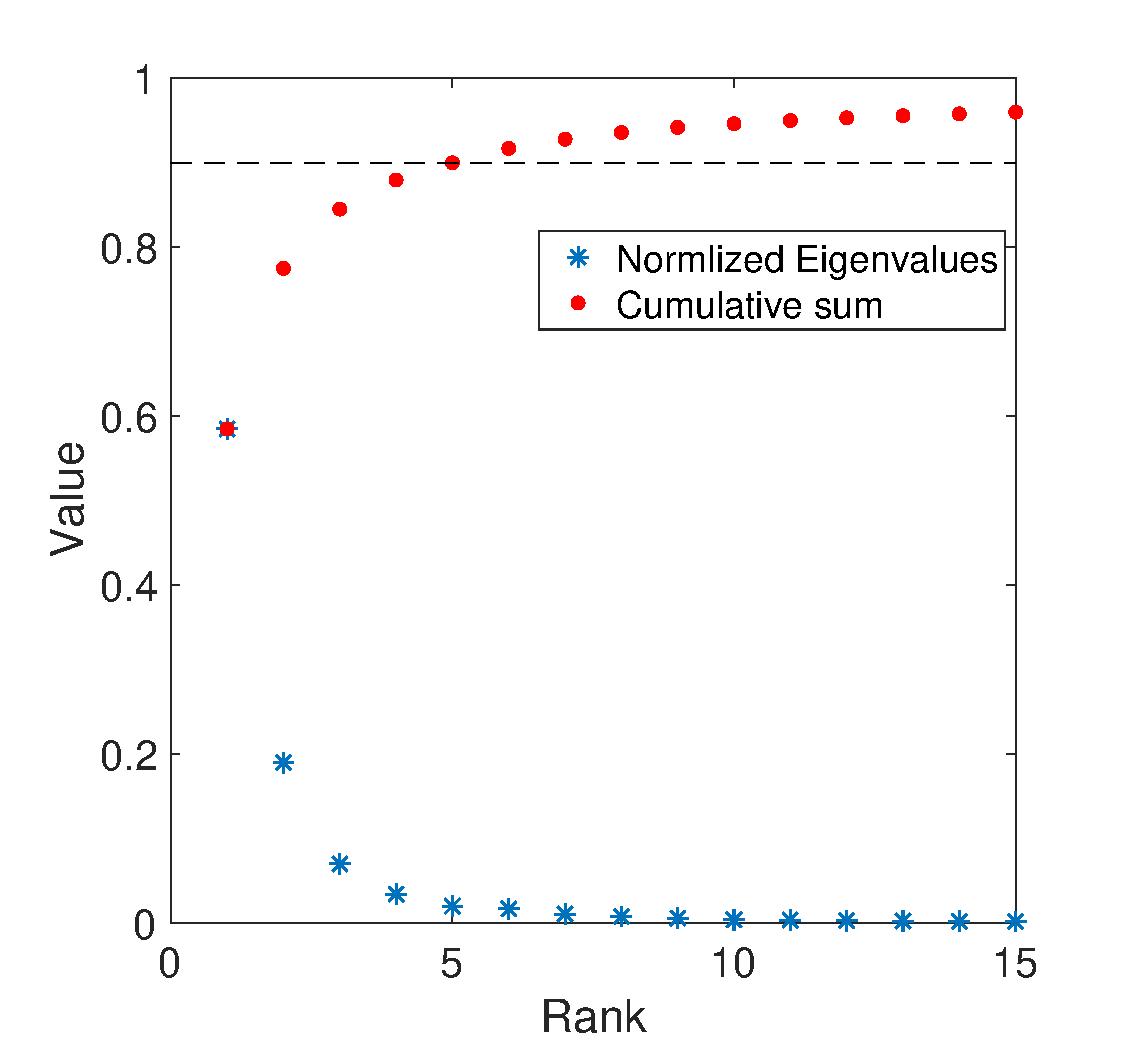
\includegraphics[width=\textwidth]{../Figures/Figure6/Figure6_e.pdf}
        \caption{xy chromaticity diagram}
        \label{fig:xyDiagram}
    \end{subfigure}
      	\begin{subfigure}[b]{0.3 \textwidth}
    \centering
        
\includegraphics[width=\textwidth]{../Figures/Figure6/Figure6_f.pdf}
        \caption{sRGB rendition of samples from Fig.~\ref{fig:randomIlluminant}}
        \label{fig:sRGBIlluminant}
    \end{subfigure}
    \caption{{\bf Generating random illumination spectra:} The illumination spectra are generated by random sampling based on the Granada daylight measurements, assuming a multivariate Gaussian distribution of weights in a 6-dimensional PCA representation. The mean and covariance matrix of the Gaussian are chosen by projecting the dataset along the first six PCA directions and taking the mean and covariance matrix of the resulting basis vector weights. (a) The 2600 spectra from the Granada natural daylight dataset, plotted on a log intensity scale in arbitrary units. (b) Rescaled version of the Granada dataset. Each spectrum is rescaled so that it has a mean value (over wavelength) of one illumination. (c) Randomly samples generated using the rescaled spectra from Fig.~\ref{fig:rescaledGranada}. (d)Normalized PCA eigenvalues and cumulative sum of the normalized eigenvalues. The eigenvalues have been normalized by the sum over all eigenvalues. The dotted line at 0.9 on the y-axis is for reference. We used the eigenvectors corresponding to the first six eigenvalues in our analysis. (e) CIE xy chromaticity plot of the rescaled dataset (in Fig.~\ref{fig:rescaledGranada}) and randomly generated samples from Fig.~\ref{fig:randomIlluminant}. (f) sRGB renditions of the random illuminant samples shown in Fig.~\ref{fig:randomIlluminant}.}\label{fig:illluminationGeneration}
\end{figure}

We generate illumination spectra  through random statistical sampling of a dataset of naturally occurring illuminants, the \href{http://colorimaginglab.ugr.es/pages/Data}{Granada daylight measurements} \cite{peyvandi2016colorimetric}.  These spectra are shown on a log intensity scale in Fig.~\ref{fig:granadaSpectra}, which illustrates that the overall intensity of natural daylights varies over several orders of magnitude, and in normalized format in Fig.~\ref{fig:rescaledGranada}, which illustrates that the relative spectra also vary considerably.  In our procedure, we first approximate the spectra in the dataset using principle component analysis (PCA). We then decompose the spectra in terms of the PCA basis vectors corresponding to the 6 largest PCA eigenvalues. Next, we sample from this low 6 dimensional PCA weight space assuming that the distribution of the basis vector weights is a multivariate gaussian whose mean and covariance matrix match the sample mean and covariance obtained from the daylight dataset. Finallly, we use the sampled weights to reconstruct sampled spectra. This general method for modeling the statistical structure of daylight was introduced by Brainard \& Freeman \cite{BrainardFreeman}. Details of the procedure we used are provided below.

Let us denote the Granada dataset as $I^G_i(\lambda)$, where $\{i \in [1,M]\}$ and $M$ is the total number of spectra in the dataset. Since the measured spectra vary over several orders of magnitude in overall intensity, we rescale each spectrum by dividing it by its mean $I_i^s(\lambda) = \frac{I^G_i(\lambda)}{\int d\lambda I^G_i(\lambda)}$. For simplicity of notation, we denote wavelength $\lambda$ as a continuous variable; in the actual calculations wavelength is discretely sampled and integrals are approximated by sums.  The Granada dataset was measured at 5 nm sampling intervals between 300 and 1100 nm.  We subsampled the spectra to the 400-700 nm interval, 10 nm spacing representation used for rendering, and performed our calculations at this sampling.

The rescaled spectra $I_i^s(\lambda)$ were then mean centered for PCA by subtracting out the mean 
rescaled spectrum, $\bar{I}^{s}(\lambda)$. That mean was obtained
by taking the sample mean over all rescaled spectra in the dataset, $\bar{I}^{s}(\lambda) = \frac{1}{M}\sum_i{I_i^s(\lambda)}$. 
The resulting mean centered dataset, $I_i^{MC}(\lambda) = I_{s}(\lambda) - \bar{I}_{s}(\lambda)$
was decomposed as $I_i^{MC}(\lambda) = \sum_j w_{ij}\hat{{\bf e}}_j^{PCA}$, 
where the $\hat{{\bf e}}_j^{PCA}$ are the PCA basis vectors obtained using the
singular value decomposition (SVD) applied to the $I_i^{MC}(\lambda)$ and
the $w_{ij}$ are the weights obtained by projecting each of $I_i^{MC}(\lambda)$ onto the  $\hat{{\bf e}}_j^{PCA}$ $\left( w_{ij} = I_i^{\rm MC}(\lambda)\cdot {\bf \hat{e}}_j^{\rm PCA}\right)$.
We used the basis vectors corresponding to
the largest six SVD eigenvalues, so that $\{j \in [1,6]\}$.
For the rescaled Granada dataset, these six  eigenvalues account for more than $90\%$ of the variance (Fig.~\ref{fig:granadaEV}).
These steps
can be summarized as follows:
\begin{align}
I^G_i(\lambda) \rightarrow I_i^s(\lambda) = \frac{I^G_i(\lambda)}{\int d\lambda I^G_i(\lambda)} \rightarrow I_i^{MC}(\lambda) = I_{s}(\lambda) - \bar{I}_{s}(\lambda) \rightarrow I_i^{MC}(\lambda) \approx \sum_{j = 1}^6 w_{ij}\hat{{\bf e}}_j^{PCA}.
\end{align}

To generate random illuminant spectra $\tilde{I}_i(\lambda)$, we generate weights $\tilde{w}_{ij}$ drawn from random 
the multivariate 
Gaussian distribution with mean $\bar{w}_j = \frac{1}{M}\sum_i w_{ij}$, 
and co-variance $\Sigma_{jj'} = \frac{1}{M} \sum_i \left(w_{ij} -\bar{w}_j\right)\left(w_{ij'} -\bar{w}_{j'}\right) $.
From these weights, the corresponding spectrum $\left( \sum_j \tilde{w}_{ij} \hat{{\bf e}}_j^{PCA} +  \bar{I}_{s} (\lambda)\right)$ is generated.
This spectrum can sometimes have values that are less than zero.  In such cases, the weights are discarded and a new draw obtained, until
the condition $\left( \sum_j \tilde{w}_{ij} \hat{{\bf e}}_j^{PCA} +  \bar{I}_{s} (\lambda)\right) > 0$, is satisfied for all $\lambda$.
The random illuminant spectrum is then given as
\begin{align}
\tilde{I}(\lambda) = \left( \tilde{I}_{MC}(\lambda) + \bar{I}_{s}(\lambda)\right).
\end{align}
Fig.~\ref{fig:randomIlluminant} shows a set of 100 spectra sampled in this manner, and may be compared with Fig.~\ref{fig:rescaledGranada}.  Fig.~\ref{fig:xyDiagram} shows the CIE xy chromaticities of these samples and compares these with the chromaticities in the Granada dataset.  Finally, Fig.~\ref{fig:sRGBIlluminant} provides an sRGB rendering of each spectrum in Fig.~\ref{fig:rescaledGranada}, to provide a visual sense of the chromatic variation in the sampled spectra.

Because our multivariate Gaussian model is based on the rescaled spectra, it does not embody the large variation in overall intensity of natural daylights.
To get a scaling similar to the original Granada spectrum set, we multiply the randomly sampled spectrum with a random number generated uniformly from the interval [0, $\bar{I}_{\rm max}$], where $\bar{I}_{\rm max}$ is the maximum of the 2600 mean values obtained from the Granada spectra. Finally, to model the fact that illumination spectra can vary in overall intensity, we draw a random number distributed logarithmically in the range [$I_{min}$ and $I_{max}$] and scale the generated spectrum by this number.
In most of our calculations, we set $I_{min} = 1$ and $I_{max} = 300$.
% WE NEED TO RETHINK THIS SCALING.  CERTAINLY SHOULD JUST BE ONE STEP.  ONE APPROACH WOULD BE TO DRAW UNIFORMLY FROM THE DISTRIBUTION OF SCALE FACTORS OBTAINED FROM THE 2600 
% GRANADA MEASUREMENTS.

\subsubsection{Surface Reflectance Spectra}

% Figure 7
\begin{figure}
\centering
	\begin{subfigure}[b]{0.3 \textwidth}
    \centering
        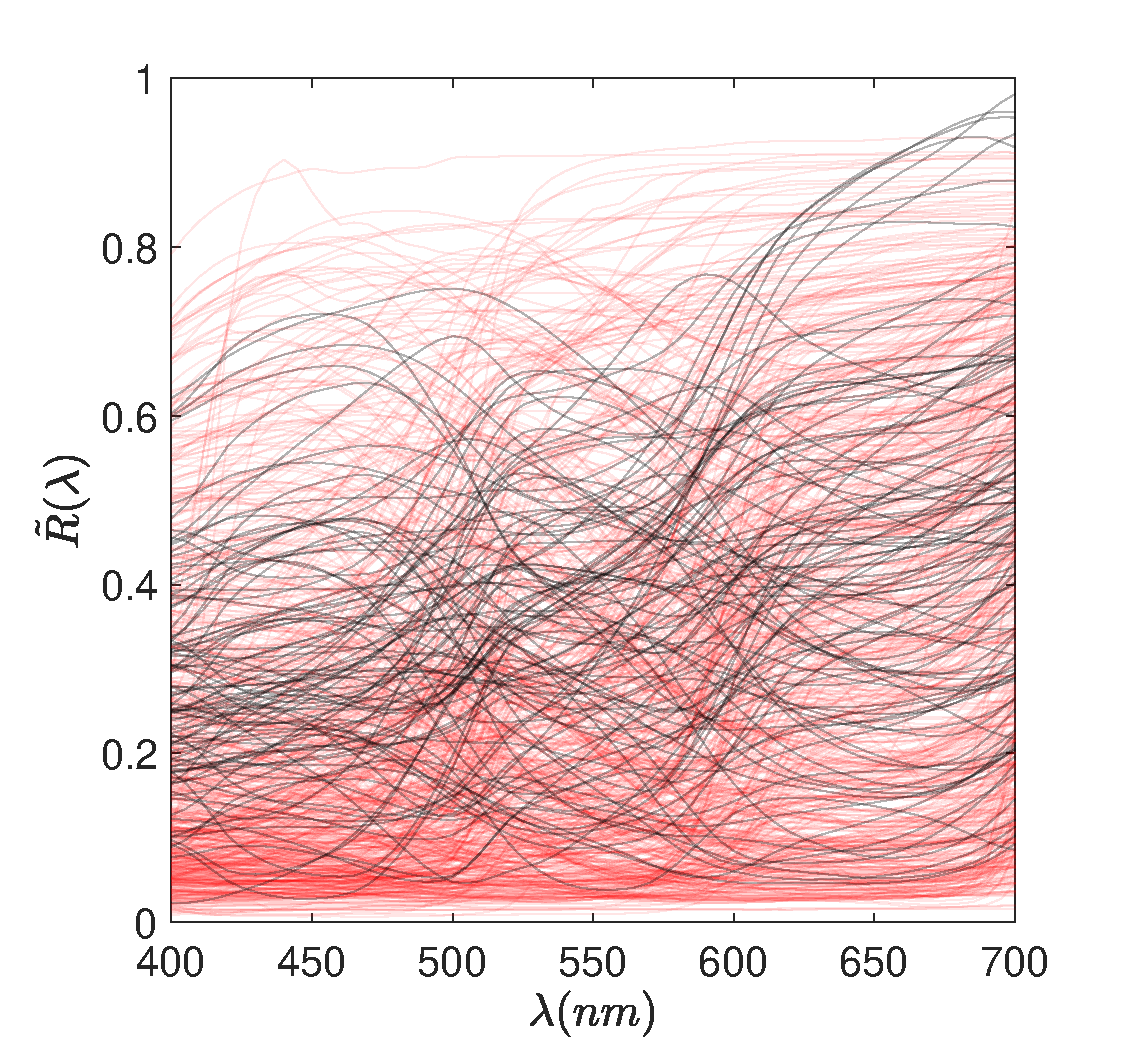
\includegraphics[width=\textwidth]{../Figures/Figure7/Figure7_a.pdf}
        \caption{Natural surface reflectance spectra}
        \label{fig:naturalSurface}
    \end{subfigure}
    \begin{subfigure}[b]{0.3\textwidth}
    \centering
        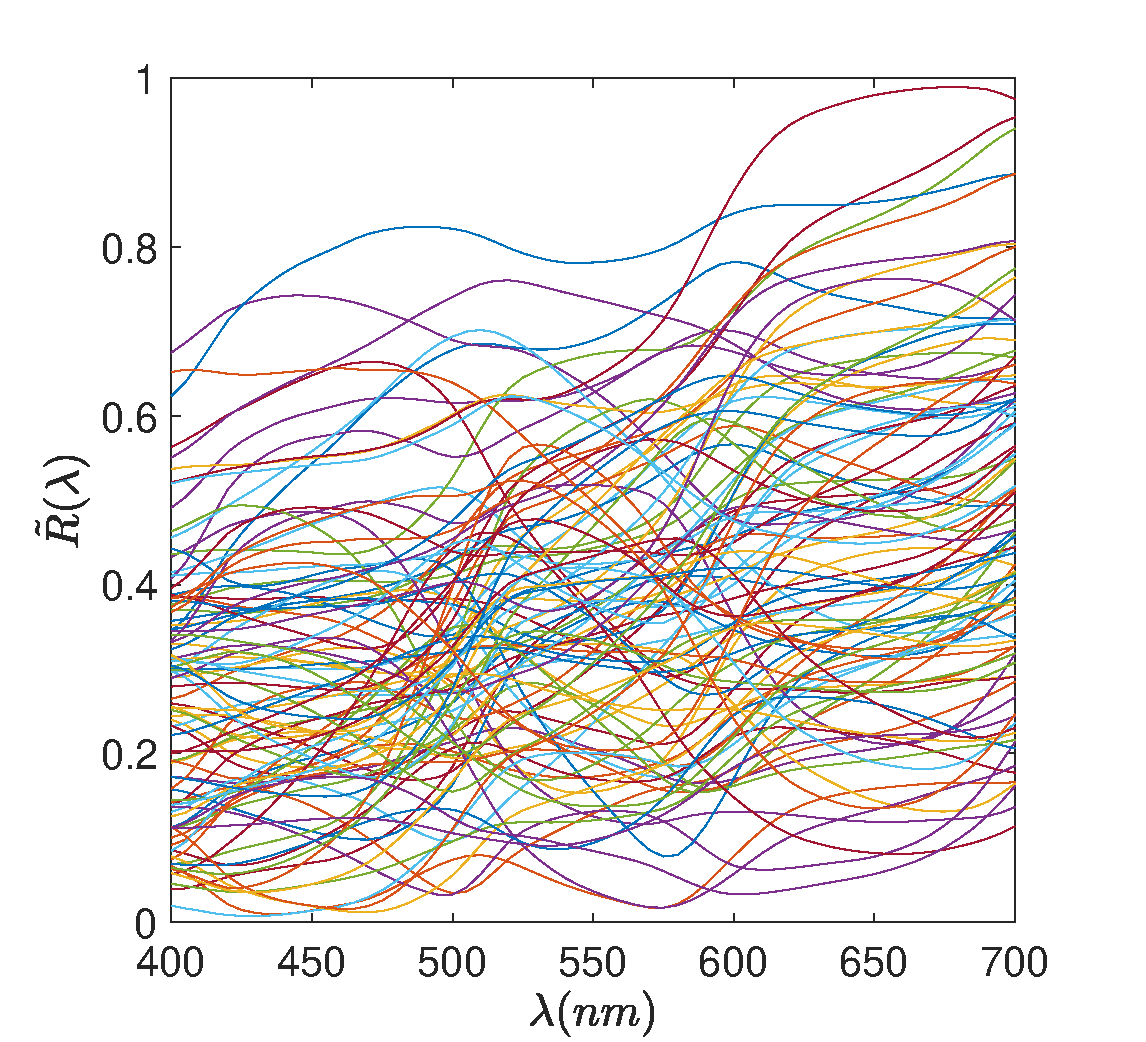
\includegraphics[width=\textwidth]{../Figures/Figure7/Figure7_b.pdf}
        \caption{Randomly generated spectra}
        \label{fig:randomSurface}
    \end{subfigure}
    \begin{subfigure}[b]{0.3 \textwidth}
    \centering
        
\includegraphics[width=\textwidth]{../Figures/Figure7/Figure7_c.pdf}
        \caption{sRGB rendition of samples from \ref{fig:randomSurface}}
        \label{fig:sRGBSurface}
    \end{subfigure}
    
    \centering
	\begin{subfigure}[b]{0.3 \textwidth}
    \centering
        
\includegraphics[width=\textwidth]{../Figures/Figure7/Figure7_d.pdf}
        \caption{Natural surface reflectance spectra}
        \label{fig:naturalSurfaceTarget}
    \end{subfigure}
    \begin{subfigure}[b]{0.3\textwidth}
    \centering
        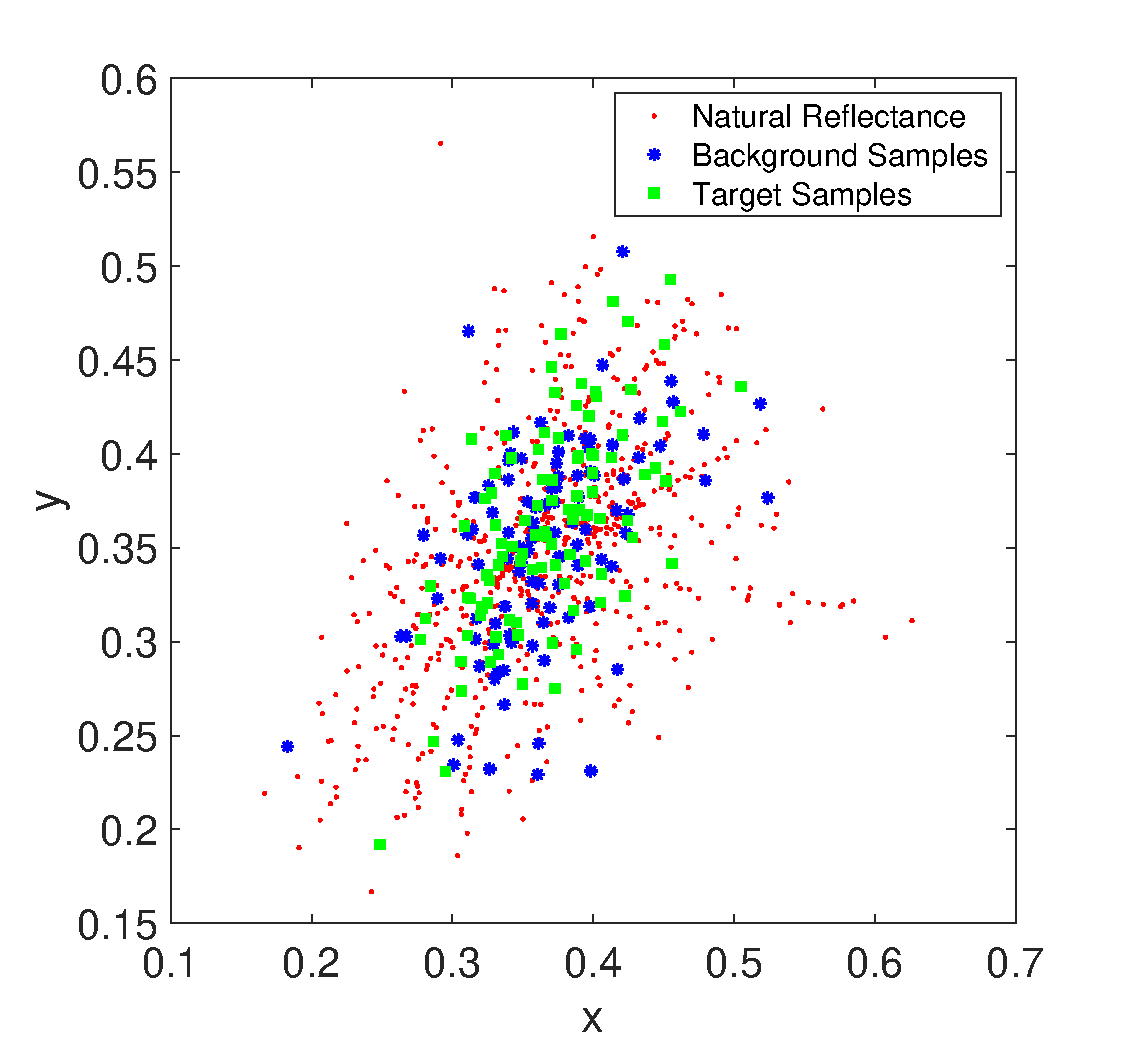
\includegraphics[width=\textwidth]{../Figures/Figure7/Figure7_e.pdf}
        \caption{Randomly generated target samples}
        \label{fig:randomSurfaceTarget}
    \end{subfigure}
    \begin{subfigure}[b]{0.3 \textwidth}
    \centering
        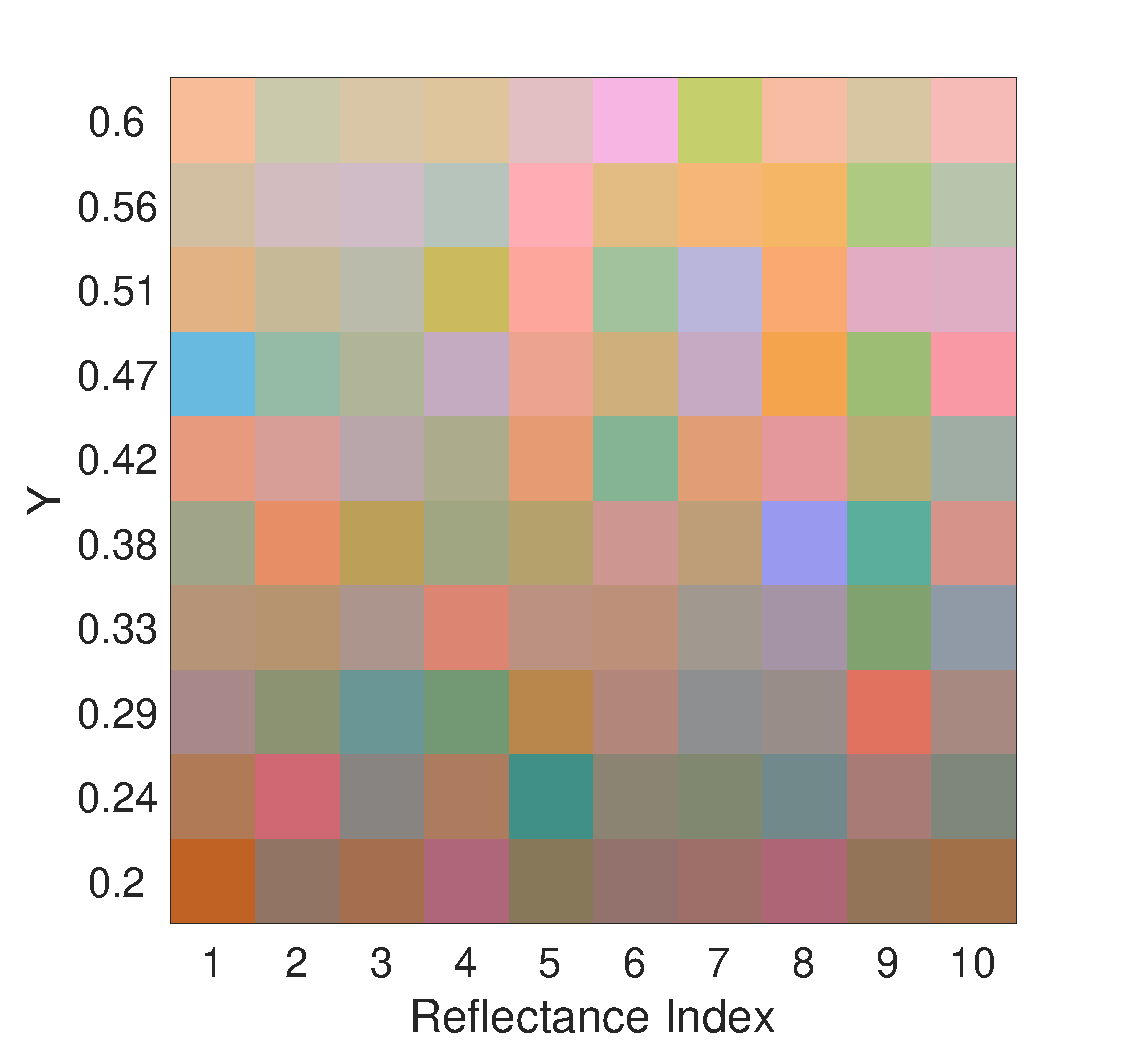
\includegraphics[width=\textwidth]{../Figures/Figure7/Figure7_f.pdf}
        \caption{sRGB rendition of target reflectance}
        \label{fig:sRGBSurfaceTarget}
    \end{subfigure}
    \caption{{\bf Generating surface reflectance spectra:} Surface reflectance spectra are generated by random sampling based on measured surface reflectance spectra, using principles similar to those used to generate random illuminant spectra. (a) The 632 surface reflectance spectra from the Munsell and Vrhel datasets. (b) Randomly generated samples of reflectance spectra. (c) sRGB renderings (under CIE D65) of the random samples generated in \ref{fig:randomSurface}. (d)Normalized PCA eigenvalues and cumulative sum of the normalized eigenvalues for the mean centered surface reflectance dataset. The eigenvalues have been normalized by the sum over all eigenvalues. The dotted line at 0.9 on the y-axis is for reference. We used the first six eigenvectors in our analysis. (e) CIE xy chromaticity plot of the surface reflectance dataset (Fig.~\ref{fig:naturalSurface}), randomly generated samples of surface reflectance (Fig.~\ref{fig:randomSurface}) and randomly generated samples of target surface. (f) The sRGB renditions of the randomly generated sample of target object surface reflectance. The figure shows 10 randomly generated samples at 10 levels of the target object surface luminance. The range of luminance levels [0.2, 0.6] (indicated on the Y axis), captures the luminance of more than 90\% of the natural surface reflectances.}
\label{fig:surfaceReflectanceGeneration}
\end{figure}

We generated random reflectance spectra using the same principles we applied to generate random illuminant spectra.
We combined the Munsell \cite{kelly1943tristimulus} and Vrhel \cite{vrhel1994measurement} surface reflectance 
measurements to create a reflectance database containing 632 reflectances. The Munsell database contains 462 samples of surface reflectance spectra each measured at 5nm sampling intervals between 380nm and 780nm. The Vrhel dataset has 170 samples measured at 2nm sampling between 390nm and 730 nm. We subsampled these spectra in the 400-700nm interval, 10 nm apart, for rendering images used in this work.

Let us denote the reflectance dataset as $R_i(\lambda)$, where $\{i \in [1,M]\}$ 
and $M$ is the total number of spectra in the dataset. 
We calculated the mean reflectance spectrum,
$\bar{R}(\lambda)$, by taking the sample mean over all spectra in the dataset, i.e.,
$\bar{R}(\lambda) = \frac{1}{M} \sum_{i=1}^M R_i(\lambda)$. Then, we mean centered 
the reflectance dataset by subtracting the mean spectrum, $R_i^{\rm MC}(\lambda) =  R_i(\lambda)-\bar{R}(\lambda)$. 
We decomposed this mean centered dataset as $R_i^{\rm MC}(\lambda) = \sum_j{w_{ij} \; {\bf \hat{e}}_j^{\rm PCA}}$, where
the ${\bf \hat{e}}_j^{\rm PCA}$s are PCA basis vectors obtained using SVD applied to $R_i^{\rm MC}(\lambda)$
and the $w_{ij}$ are the weights obtained by projecting each of $R_i^{\rm MC}(\lambda)$ onto the basis vectors ${\bf \hat{e}}_j^{\rm PCA}$ 
$\left( w_{ij} = R_i^{\rm MC}(\lambda)\cdot {\bf \hat{e}}_j^{\rm PCA}\right)$. 
We used the basis vectors corresponding to the largest six SVD eigenvalues. 
For the combined Munsell and Vrhel datasets, these six eigenvalues account for 
more than $90\%$ of the variance. 
To generate random reflectance spectra, we generate samples of weights ($\tilde{w}_{ij}$) drawn from the multivariate Gaussian 
distribution with mean $\bar{w}_j = \frac{1}{M}\sum_i w_{ij}$, 
and co-variance $\Sigma_{jj'} = \frac{1}{M} \sum_i \left(w_{ij} -\bar{w}_j\right)\left(w_{ij'} -\bar{w}_{j'}\right) $. If the randomly sampled weights satisfy the condition $\left( 0 < \sum_j \tilde{w}_{ij}{\bf \hat{e}}_j^{\rm PCA} + \bar{R}(\lambda)<1\right) $ at every $\lambda$, we use them to give the random reflectance spectrum as: $\tilde{R}_i(\lambda) =\sum_j \tilde{w}_{ij}{\bf \hat{e}}_j^{\rm PCA} + \bar{R}(\lambda)$.  Otherwise the draw is discarded and a new set of weights is drawn.

For generating the target object reflectance at a particular luminance $(Y_{\rm T})$, the values in a generated spectrum were 
rescaled such that the surface luminance (as defined above) had the desired value.
The scaling equals $\frac{Y_{\rm T}}{\int d\lambda \tilde{R}(\lambda) D_{65}(\lambda) \bar{y}(\lambda)}$, with $\bar{y}(\lambda)$ being the CIE photopic luminosity (or luminous efficiency) function. 
$\bar{y}(\lambda)$ describes the average spectral sensitivity of human visual 
perception of bruminance. The target reflectance is then given by: $\tilde{R}^{\rm T}_i(\lambda) =\tilde{R}_i(\lambda) \cdot\left(\frac{Y_{\rm T}}{\int d\lambda \tilde{R}(\lambda) D_{65}(\lambda) \bar{y}(\lambda)}\right)$.

% Figure 8: Methods
\begin{figure}
\centering
\begin{subfigure}[b]{0.25 \textwidth}
		\centering
        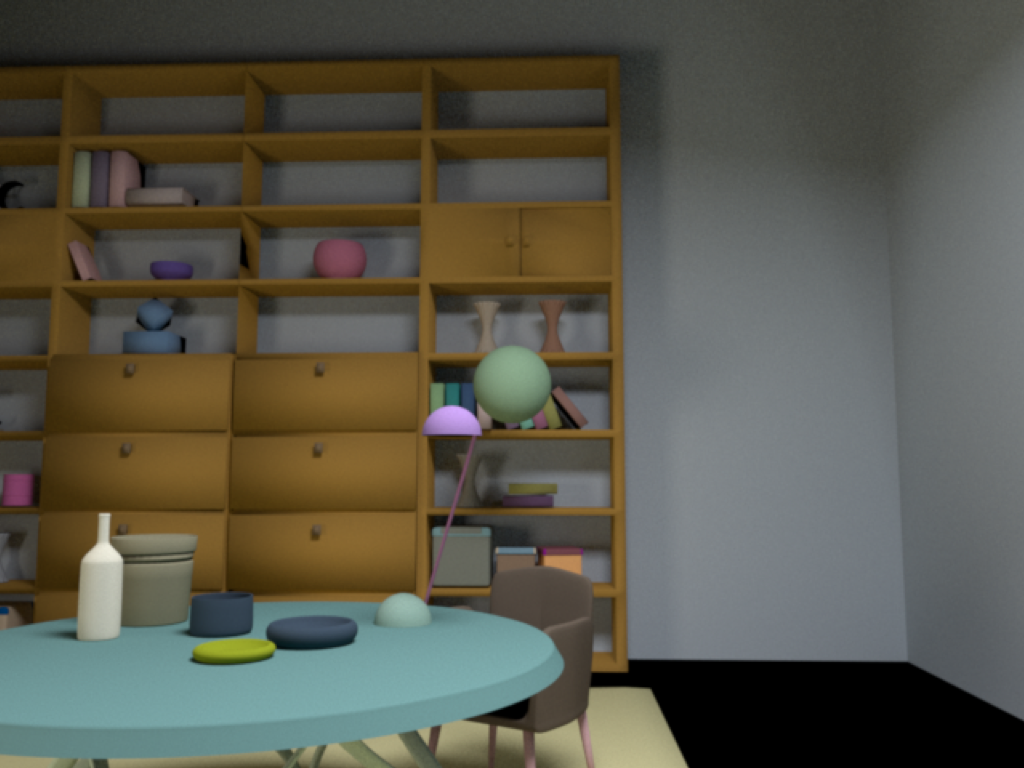
\includegraphics[width=\textwidth]{../Figures/Figure8/Figure8_a.png}
        \caption{sRGB rendering of a 3D scene}
        \label{fig:3DScene}
    \end{subfigure}
    ~ 
    \begin{subfigure}[b]{0.19 \textwidth}   
    \hspace{0.1 \textwidth}
        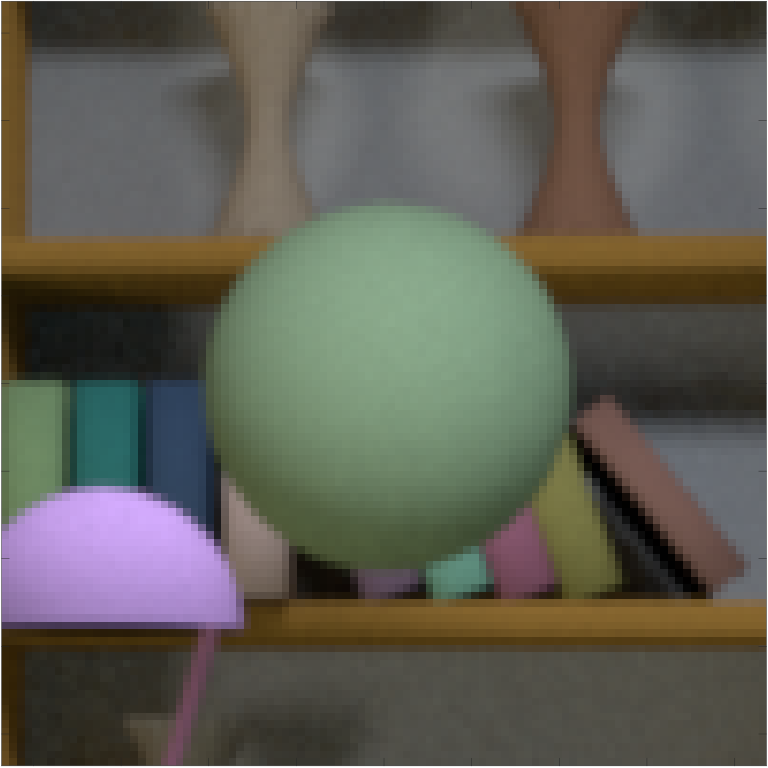
\includegraphics[width=\textwidth]{../Figures/Figure8/Figure8_b.png}
        \caption{Cropped Image}
        \label{fig:croppedImage}
    \end{subfigure}
    ~ 
    \begin{subfigure}[b]{0.19 \textwidth}
    \hspace{0.1 \textwidth}
        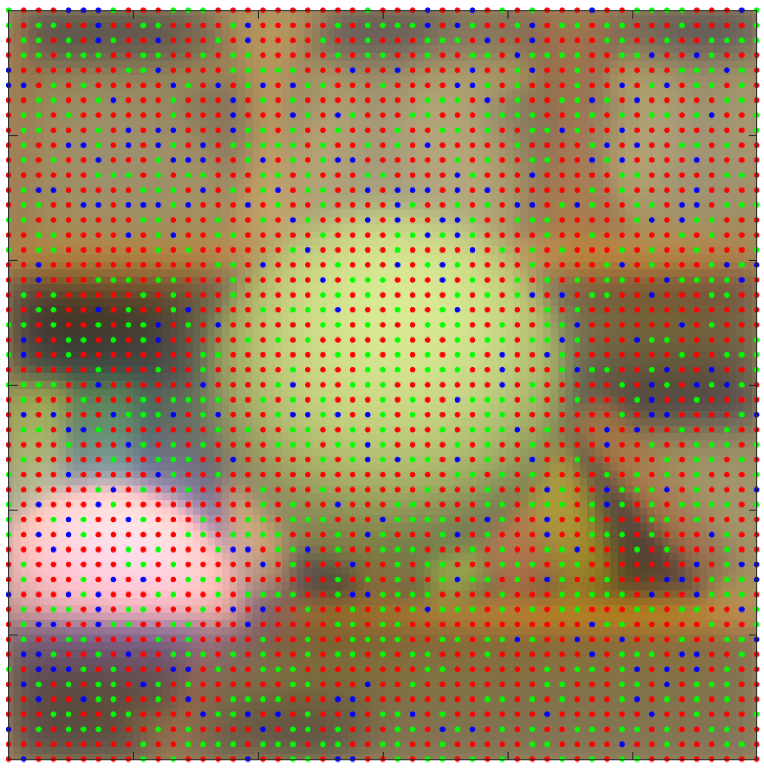
\includegraphics[width=\textwidth]{../Figures/Figure8/Figure8_c.png}
        \caption{Optical Image}
        \label{fig:croppedImageWithMosaic}
    \end{subfigure}
    ~
    \begin{subfigure}[b]{0.2 \textwidth}
        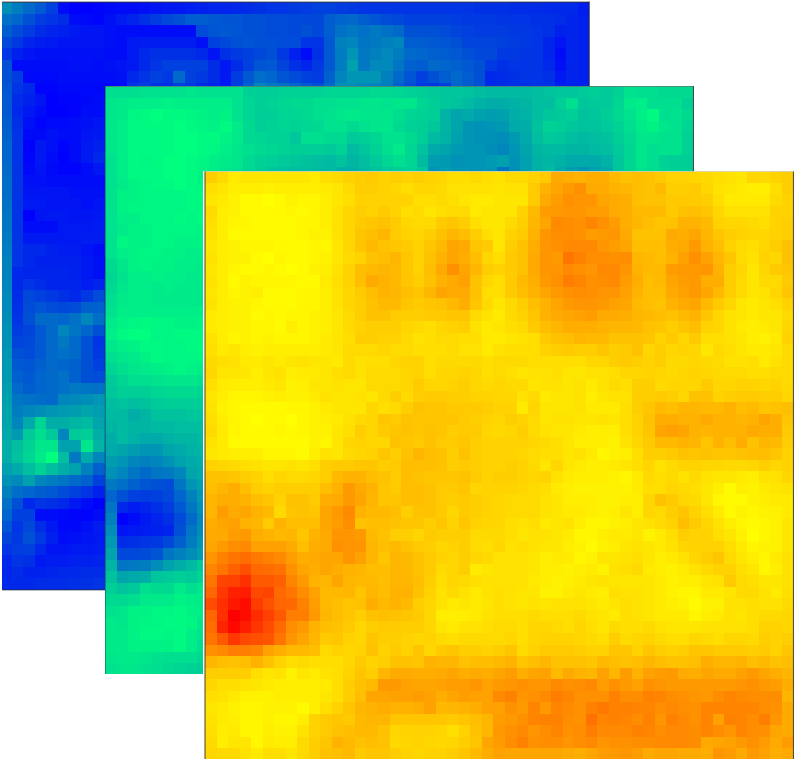
\includegraphics[width=\textwidth]{../Figures/Figure8/Figure8_d.png}
        \caption{LMS cone contrast}
        \label{fig:coneContrast}
    \end{subfigure}
    \label{fig:sceneWithCroppedImage}
    \caption{{\bf Generating labeled dataset for computational analysis:}  For the supervised approach employed in this work, the labeled database is generated as follows: (a) A 3D virtual scene, containing a target object of known surface luminance is created. The target object is placed in the camera field of view. After assigning spectra to the light sources and other other objects in the scene, a multispectral image of the scene is rendered using the Mitsuba software package. (b) The central portion of the rendered image, which contains the target object, is cropped from the image. (c) The response of retinal cones to the cropped image is simulated using the isetbio software package to model early vision. The software models optical blurring and foveal spatial sampling by the trichromatic cone mosaic. Fig.~\ref{fig:croppedImageWithMosaic} shows the retinal image incident on the cone mosaic and the location and the identity of the cones (L cones: Red, M cones: Green, S cones: Blue).  (d) The cone responses are interpolated to estimate the responses of all the three types of cone at each location (demosaicing). Finally, the demosaiced images are contrast normalized separately for each cone type.}
\end{figure}

\subsection{Model of Early Visual System} \label{method:Isetbio}

The sampling and rendering steps described above allow us to generate images from scenes that contain an image of a target object of known surface luminance at the center pixel, and where the illuminant spectra and spectra of the other surfaces in the scene are drawn randomly from models of naturally occurring spectra.  One such image is shown in Fig.~\ref{fig:3DScene}, where the green sphere in the middle is the target object and the light sources are not within the camera field of view. We model the encoding of such images by the early visual system, to generate {\em neural images} that provide an abstracted representation of the information available to the brain for producing perceptual representations of the external world. For each image, it is this information together with the known surface luminance of the corresponding target object that we will provide to our supervised learning algorithms.  Our training datasets correspond to ... % SAY WHAT WE DID ONCE WE FINISH EVERYTHING OFF.

In this work, we are interested in how well luminance constancy may be achieved using information that is local to the image region containing the target object. 
To analyze the local image information, we cropped and processed the image in the immediate neighborhood of the target object such that each patch represented a one degree of visual angle, approximately the size of a receptive field in early visual cortex (\ref{fig:croppedImage}).
Fig. \ref{fig:studiedCases} shows examples of such cropped image at 3 luminance levels for the three cases considered in this paper.
Next, the cropped multispectral images are used to simulate retinal cone responses using \href{https://github.com/isetbio}{Isetbio} software. The key steps we model are the size of the pupil, optical blurring (including axial chromatic aberration) in the formation of the retinal image, spatial sampling by an interleaved mosaic of long (L), middle (M)  and short (S) wavelength-sensitive cones, and the Poisson nature of photopigment isomerization.
We use the multispectral cropped image (Fig.~\ref{fig:croppedImage}) as the optical stimulus to simulate the response of the cones in the retina. The cropped image patch is assumed to cover a $1^{\circ}$ field of view at a distance of 1 m. The retinal cone mosaic is modeled as a square grid with $51 \times 51$ cones in the L:M:S ratio 0.6:0.3:0.1. The response of the cones are taken as the number of isomerizations in the cone segment ({\it over what time ??}).

% NEED TO WRITE IN THE KEY PARAMETERS USED. PROBABLY MARIMONT AND WANDELL OPTICS, STOCKMAN-SHARPE LMS CONE SPECTRAL SENSITIVITIES, THE L, M, S CONE RATIO IN THE MOSAIC, RECTANGULAR AND REGULAR CONE PACKING, SOME IMPLIED SPATIAL SCALE, AND SOME OVERALL SCALING THAT DRIVES THE MEAN LUMINANCE OF THE RETINAL IMAGES AND THUS THE AMOUNT OF POISSON NOISE. ALSO INTEGRATION TIME.
The cone response functions are normalized by the total area under the response curves to model the amplification of the S cone response downstream and thus have comparable number if isomerizations in L, M and S cones. 
% NEED TO UNDERSTAND THIS.  WHEN WAS THE GAIN, BEFORE OR AFTER NOISE ADDED, AND LET'S REMEMBER WHY WE DID IT.  
% First we add noise, then we do the scaling. The reason this was done is to make sure that in the normalization process each of the cone class have the same contribution. Otherwise, the S cone contribution would be very low.

The cone isomerizations represent the first step of visual processing.  To capture key properties of post-receptoral processing, such as contrast normalization (REFS),
% Heeger 1992, Albrecht and Geisler 1991 (contrast normalization)
% Carindini Heeger 2012 (Review on contrast norm)
we processed the isomerizations as follows:
First, we created a representation for each cone class on the full $51 \times 51$ pixel grid, we interpolated the responses of the cones in each class across the grid, using bilinear interpolation separately for each cone class.
% DOUBLE CHECK THAT THIS WAS DONE WITH SOMETHING LIKE INTERP2 WITH THE LINEAR OPTION.
This gives us a $51 \times 51$ cone response image for each cone class.
The three $51 \times 51$ sets of cone responses corresponding to the L, M and S cones were then reshaped into a single $7803 \times 1$ vector ($7803 = 51 \times 51 \times 3$). For case 1 and 3 we used this as the input for the supervised methods. For case 3 and 4, to model the contrast coding and contrast adaptation, we convert this vector to a contrast representation by subtracting out the mean and then dividing by it (contrast coding), followed by normalizing the vector to have unit length (contrast normalization).
The cone-response vectors corresponding to the N images for each case are concatenated column-wise to form a contrast normalized matrix $C_{7803\times N}$. The corresponding labels are represented by the row vector $Y_{1\times N}$.

\subsection{Supervised Learning methods} \label{method:SupervisedLearning}
We have two supervised learning methods in our work: Linear regression and Accuracy maximization analysis. While, our main focus is on AMA, linear regression provides a baseline performance measure.

\subsubsection*{Linear Regression} For linear regression, we solve the equation $A_{1\times3}*C_{3\times N} = Y_{1\times N}$ for the regression parameters $A_{1\times3}$. Here, $C_{3\times N}$ is a matrix containing either the L, M and S cone responses (for case 1 and 2) or contrast normalized responses (for case 3 and 4) of the central patch of each image, extracted from $C_{7803\times N}$.  The columns corresponds to the N images in the dataset. The rows correspond to the contrast normalized L, M and S cones responses averaged over a 3$\times$3 pixel central region of the image containing the target object.  The (unknown) regression parameters $A$ are obtained using Matlab linear regression function. This model provides a baseline performance measure, which does not take the context in which the target image is seen into account.

\subsubsection*{Accuracy maximization analysis}
We perform two steps to decode the luminance of the target object from the cone isomerization. First, we use AMA to learn the linear filters that are optimal for estimating the target object luminance. Second, we determine how to optimally decode the luminance from the response of these filters to arbitrary stimuli.

{\bf Learning optimal filters using AMA:} AMA \cite{geisler2009optimal,burge2017accuracy}
% add Jaini burge 2017
is a task specific Bayesian method for dimensionality reduction. When provided with a labeled training set, a receptive field response model, a decoder that uses these responses to estimate the stimulus label, and a cost function, AMA returns the linear receptive fields (in rank order) that are optimal for performing a task. The optimal receptive fields that are returned by AMA are those whose responses to the stimuli minimizes the cost function over the training set when optimally decoded. 

More concretely, let us assume that there are $N_{\nu}$ possible values of the target object luminance levels ($\{Y_k: k\in[1,N_{\nu}] \}$) and the $l$'th image corresponding to the $k$'th luminance level is represented as $s_{kl}$. Also, assume that there is a set of linear receptive fields {\textbf{\textit f}} which when acting on $s_{kl}$ gives the response ${\textbf{\textit R}}_{kl}$. Also assume there is a decoder $g$, with the knowledge of the response model and of every stimulus in the training set, that returns the Bayes' optimal estimate of the luminance level ($\hat{Y}_k$) of the target object in each stimulus $s_{kl}$. The crux computation for obtaining this estimate is the computation of the posterior probability of the luminance given an observed response, $P(Y|\textbf{R}_{kl})$ \cite{geisler2009optimal,burge2017accuracy}
% add Jaini burge 2017
. With this luminance estimate, we calculate the cost given the cost function $\mathcal{C}_{kl} = \gamma(Y_{kl},\hat{Y}_{kl})$. Finally, AMA searches for the set of optimal receptive fields ${\textbf{\textit f}}^{\rm opt}$ that minimize the cost over the entire training set $\{s_{kl}: k\in[1,N_{\nu}], l\in[1,N_k]\}$ where $N_{k}$ is the number of stimuli corresponding to the label $Y_k$. Thus,
\begin{align}
{\textbf {\textit f} }^{\rm opt} = \argmin_{\textbf {\textit f} } \sum_{k=1}^{N_{\nu}}  \sum_{l=1}^{N_k} {\mathcal{C}}_{kl}.
\label{eq:fopt}
\end{align}

{\bf Estimating luminance:} 
Once the optimal receptive fields have been learned, a general decoder must be used to estimate the luminance. Recall that the decoder used to learn the receptive fields required the knowledge of every stimulus in the training set. To obtain the general decoder, first we use the AMA optimal receptive fields and the training dataset to find the conditional distributions of the AMA receptive field responses $P({\textbf {\textit R} }|Y_i)$. Then, we approximate these with multivariate Gaussian distributions $P({\textbf {\textit R} }|Y_i) = \mathcal{N}\left(\mu(Y_i),\Sigma(Y_i) \right)$. To estimate the luminance of the target object in the test stimulus, we use Bayes' rule to obtain the posterior distribution $P(Y|{\textbf {\textit R} })$. The optimal estimate is the luminance value that minimizes the cost function.

{\bf Estimating labels:} 

Once these filters have been learned, a suitable decoding method (in this case a Bayesian decoding scheme) is used to estimate the label on a test set.

The image labels are estimated using the Bayesian decoder as described above. First, we use the AMA optimal filters and the training dataset to find the conditional distribution of the AMA filter response $p({\textbf {\textit R} }|Y_i)$. We then approximate this distribution with multivariate normal distribution $p({\textbf {\textit R} }|Y_i) = \mathcal{N}\left(\mu(Y_i),\Sigma(Y_i) \right)$. To estimate the label of an image from the test set, we use Byes' rule to obtain the posterior distribution $p(Y_i|{\textbf {\textit R} })$. The estimated value is the one that optimizes the cost function.

\subsection{Error estimation}
If $\hat{Y}$ is the estimated luminance corresponding to the assigned luminance $Y$, the error of the luminance estimates is quantified as the relative error ($E_{\rm rel}$) defined as: $E_{\rm rel}^2 = \left\langle\left((\hat{Y}-Y)/Y\right)^2\right\rangle$.


% THINGS TO THINK ABOUT:
%  1) Putting error bars on performance.  Particularly want to be sure that Fig 13 feature that Case 3 RFs do better than Case 1 RFs for Case 1 is just statistical sampling.
%  2) What exactly do we want to run for final version.  How much illuminant intensity variation?  Should we make this match psychophysics so we could imagine these images displayed on a monitor?
%  3) Do we just want to look at results for contrast normalized, or do we want to pick them off separately for isomerizations, contrast, and contrast normalized?
%  4) What is driving the response variability in Case 1, where the stimulus is basically deterministic up to noise.  There are three sources of noise: 1) Rendering noise, 2) Isomerization noise, 3) AMA noise introduced for some unknown reason, 4) Variation in target color.

% WHAT STORY DO WE WANT TO TELL ABOUT THE RESULTS
%  1) Case 0 -- work out effect of sources of internal noise - isomerization and AMA -- without any external "noise", where external "noise" is the effect of variability in object extrinsic scene factors (illumination, surrounding objects). 
%                      Also establish the rendering noise is einsy relative to whatever else we're doing.
%  2) Move to Case 1 -- what happens when we introduce color variability into the target.  This may not be of interest to the psychophysics, but none-the-less seems interesting to know as one ponders lightness constancy.
%  3) On to Case 2 -- here the question is, do we keep varying target color, or do we fix target color and vary illumination?  In any case, this isn't too hard a case if the other objects remain fixed, because then contrast coding basically normalizes out a lot of the variation, and it's only the spectral variation that might screw things up.  But, that's why we run case 3.
%  4) Do we run a case where the relative spectrum of the illuminant stays fixed and we only vary intensity?
%  4) On to Case 3 --

\section{Results} \label{Results}
In this section, we discuss the results of supervised learning to estimate the luminance of the target object on the the various cases we described previously. We describe the computations that need to be performed on the cone photoreceptor responses to estimate the luminance. We start with case 1, where only the reflectance spectrum of the target object is allowed to vary, and show that in this case the luminance can be estimated directly from the photoreceptor response. We then progressively increase the complexity of the spectral conditions and explain the correspondingly complex computations that are required to estimate the target object luminance. Next, we show the optimal AMA receptive fields for each one of the spectral cases discussed in this work. We show that the optimal receptive fields for target luminance estimation have a center surround structure and they give more weights to the response of L and M cones than S cones. We finally show that, as expected, the receptive fields for the complex spectral cases generalize to the simple cases. Hence, one requires only one set of optimal receptive fields for estimating the target luminance, not separate receptive fields for each spectral case.

\subsection{Luminance estimates for each spectral case}
\subsubsection{Case 1: Target object relative surface reflectance spectrum variable, light source and background object spectra fixed}
We started our analysis with the simplest case, where only the target object relative spectrum is allowed to change. 
We used AMA to learn a set of linear receptive fields that are optimal for estimating target object luminance for the stimuli in this case. 
Fig.~\ref{fig:case1RFResponse} shows the projection of the photoreceptor response along the first two optimal AMA receptive fields. 
Clearly, there exists a subspace along which the photoreceptor response separates according to the luminance level assigned to the target object. 
Thus, the target object luminance can be obtained by projecting photoreceptor responses along these AMA receptive fields. 
We used such projections and a generalized decoder Bayes' decoder (see methods) to estimate the luminance of the target objects in the test set stimuli.
Fig.~\ref{fig:case9Results} shows the estimated luminance v/s the actual luminance assigned to the target object for the test stimulus in case 1. 
We show the estimates obtained by AMA and two null models: a naive method that assigns the average target object luminance across the training set to all images, and a linear model based on the photoreceptors corresponding to the center pixel on the target object (see Methods). 
As expected, in the absence of any external source of variation, the photoreceptor response is proportional to the luminance of the target object, and hence can be easily estimated by both AMA and linear regression.

Each cloud in Fig.~\ref{fig:case1RFResponse} corresponds to the photoreceptor response to the images with target luminance level at a fixed value. 
The variation within the cloud, between images that have the target object at same luminance values, results due to the difference in the relative shape of the target object reflectance spectra (difference in hue and saturation). 
The resulting variation dominates any variation coming from the noise in photoreceptor response or the noisy rendering of the images by the software.
Fig.~\ref{fig:case0RFResponse} shows the projection of photoreceptor response corresponding to 1000 images where, in addition to the illumination and background spectra, we also fixed the relative shape of the target object surface reflectance. 
The variation resulting from the poisson nature of the photoreceptor response or due the image rendering software is small and can be ignored.

%% Figure 9
\begin{figure}
\centering
        \begin{subfigure}[b]{0.3 \textwidth}
        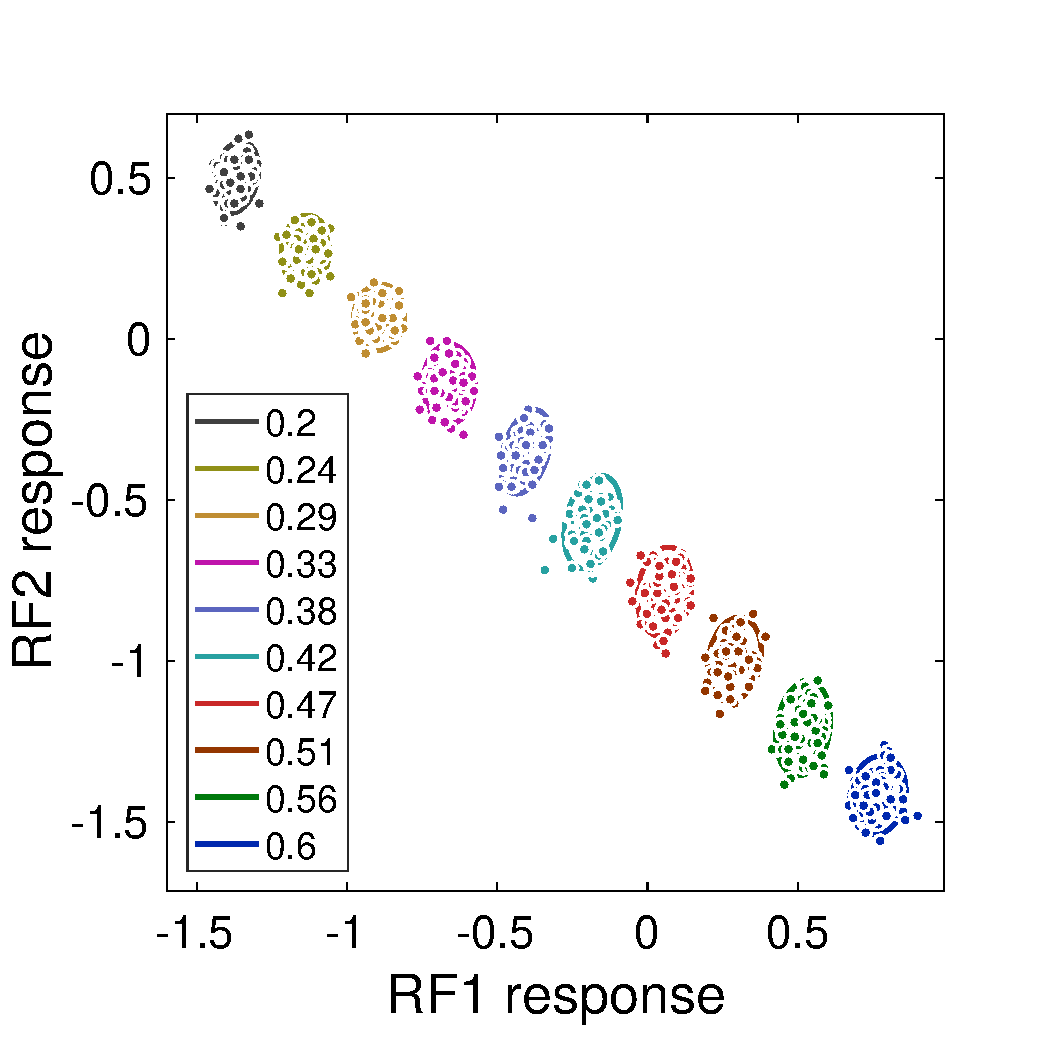
\includegraphics[width=\textwidth]{../Figures/Figure9/Figure9_a.pdf}
        \caption{RF response Case 1}
        \label{fig:case1RFResponse}
    \end{subfigure}    
%    \begin{subfigure}[b]{0.33 \textwidth}   
 %       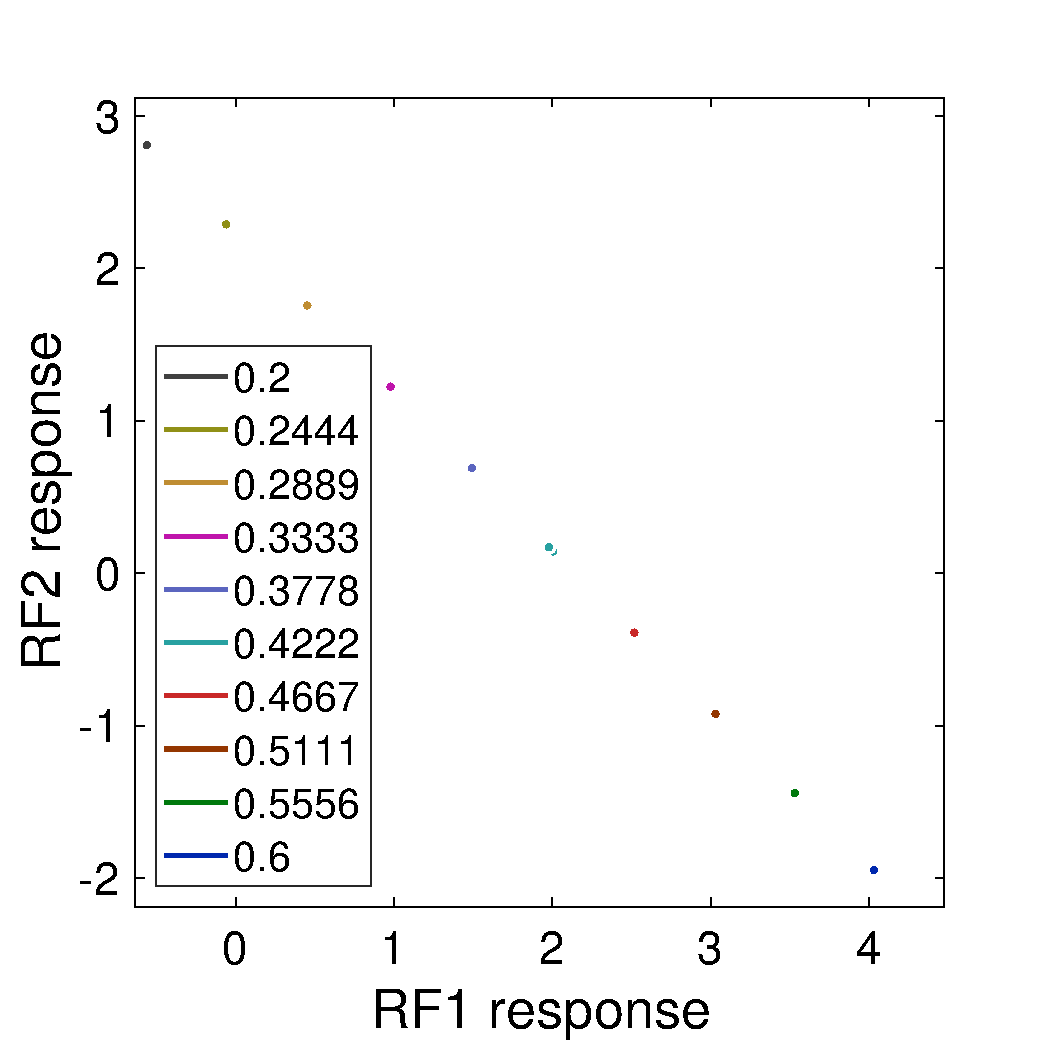
\includegraphics[width=\textwidth]{../Figures/resultsFigure/renderingNoise.pdf}
%        \caption{Rendering noise}
%        \label{fig:renderingNoise}
%    \end{subfigure}
            \begin{subfigure}[b]{0.297 \textwidth}
        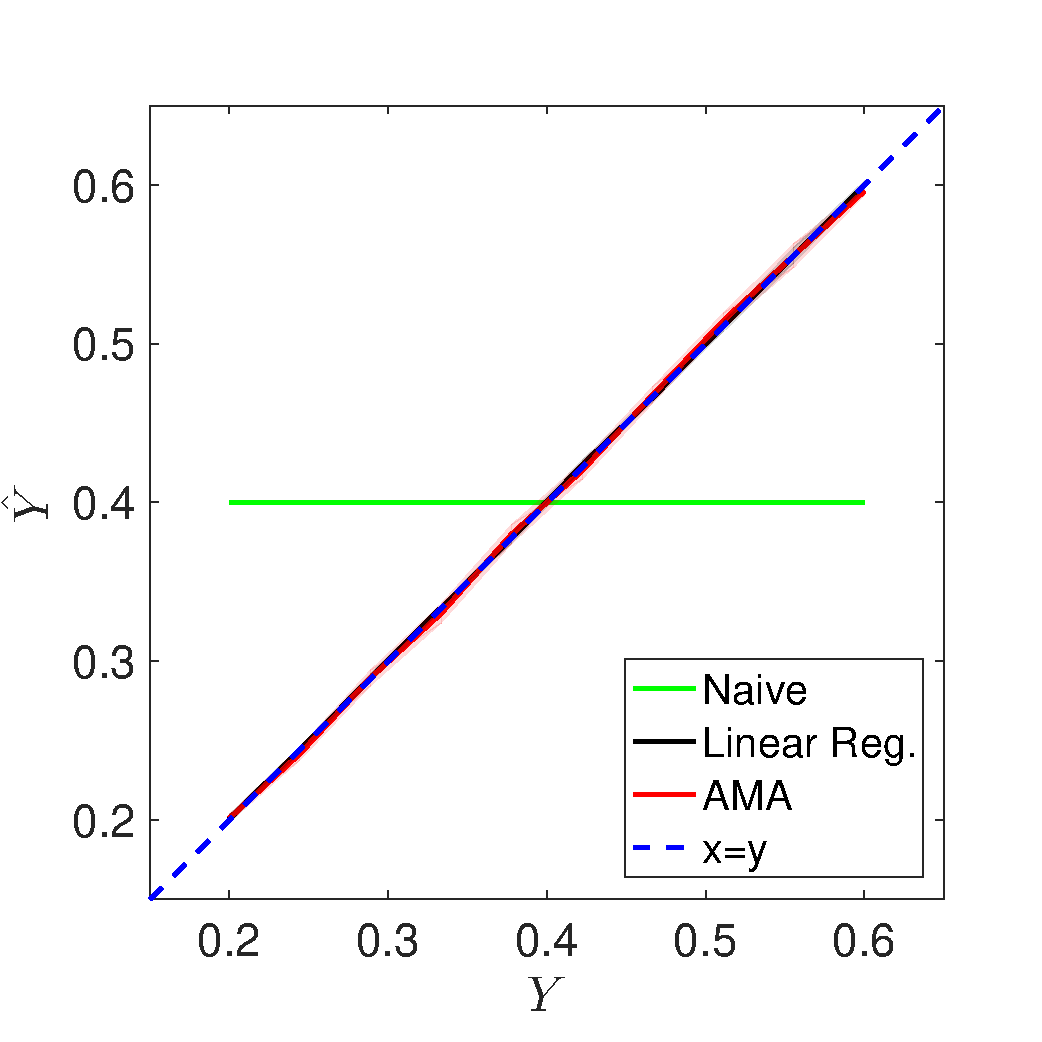
\includegraphics[width=\textwidth]{../Figures/Figure9/Figure9_b.pdf}
        \caption{Luminance Estimates}
        \label{fig:case9Results}
    \end{subfigure}    
        \begin{subfigure}[b]{0.3 \textwidth}
        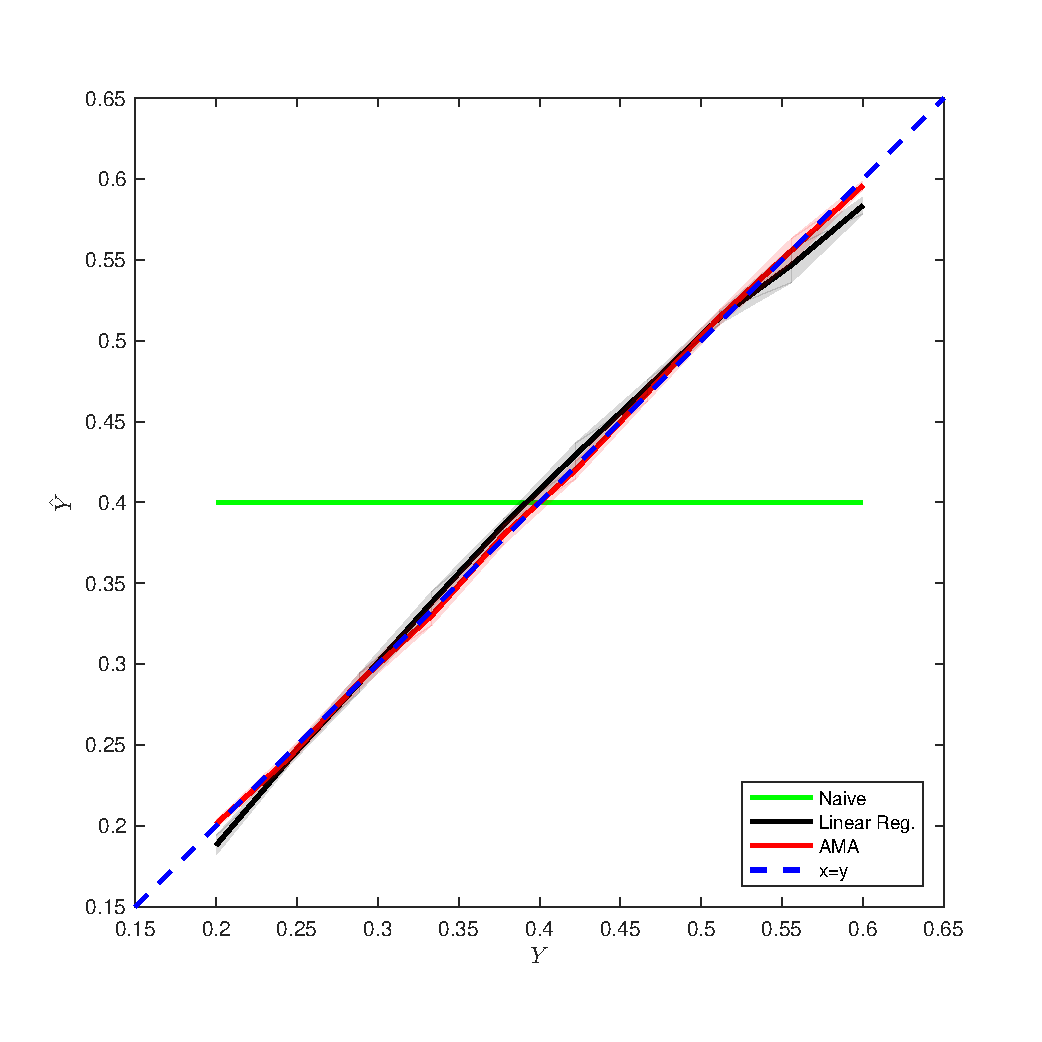
\includegraphics[width=\textwidth]{../Figures/Figure9/Figure9_c.pdf}
        \caption{Images with fixed relative spectrum}
        \label{fig:case0RFResponse}
    \end{subfigure}
    \caption{{\bf Case 1: RF response and luminance estimates:} (a) Photoreceptor response projected along the first two AMA receptive fields for images of case 1. We show the response for the images in the training set. Each response cloud represents the response of images corresponding to one luminance level. The response clouds are approximated by a multinormal Gaussian whose mean and variance are approximated by the ellipses shown in the figure. (b) Mean luminance estimates and standard deviations for the images in the test set obtained using the naive method, linear regression and AMA. The estimates fall along the diagonal unit slope line for both linear regression and AMA. The standard deviations are too small to be visible. (c) Photoreceptor response for images with fixed relative shape of the target object reflectance spectrum projected along the first two case 1 AMA receptive fields. The variation coming from the poisson nature of the photoreceptor isomerization is small compared to the variation due to shape of target object reflectance spectrum.}
\label{fig:sourcesOfNoise}
\end{figure}

\subsubsection{Case 2: Target object relative surface reflectance spectrum variable, light source spectra fixed, background object spectra variable}
Fig.~{\ref{fig:case2RFResponse}} shows the projection of the photoreceptor response for case 2 along the first two AMA receptive fields. The naive expectation would be that variations in background objects surface reflectance would have minimal effect on the isomerizations of the cones corresponding to the target object. Hence, the luminance can be estimated directly from the isomerization of these cones. But projection of the cone response along the AMA RFs shows that the background variation has significant effect on the cone isomerizations. The response clouds at different luminance levels along the first two receptive fields do not separate as well compared to case 1. The overlap is lower if the projection is considered in subspaces that have more AMA receptive fields. Fig.~\ref{fig:ErrorVsNFilters} shows the relative error of luminance estimate as a function of the number of AMA receptive fields used for luminance estimation. As expected, the relative error decreases with the number of receptive fields and converges to the minimum value around 8 receptive fields. Fig.~\ref{fig:case2Estimates} shows the luminance estimates for the learning methods used in this work. The mean estimates fall along the diagonal x=y line. The variance in the estimates increases with assigned luminance. This is because the isomerization noise is directly proportional to the light reflected from the target object and is higher at higher values of the target object luminance.

%% Figure Case 2
\begin{figure}
\centering
    \begin{subfigure}[b]{0.3	 \textwidth}   
        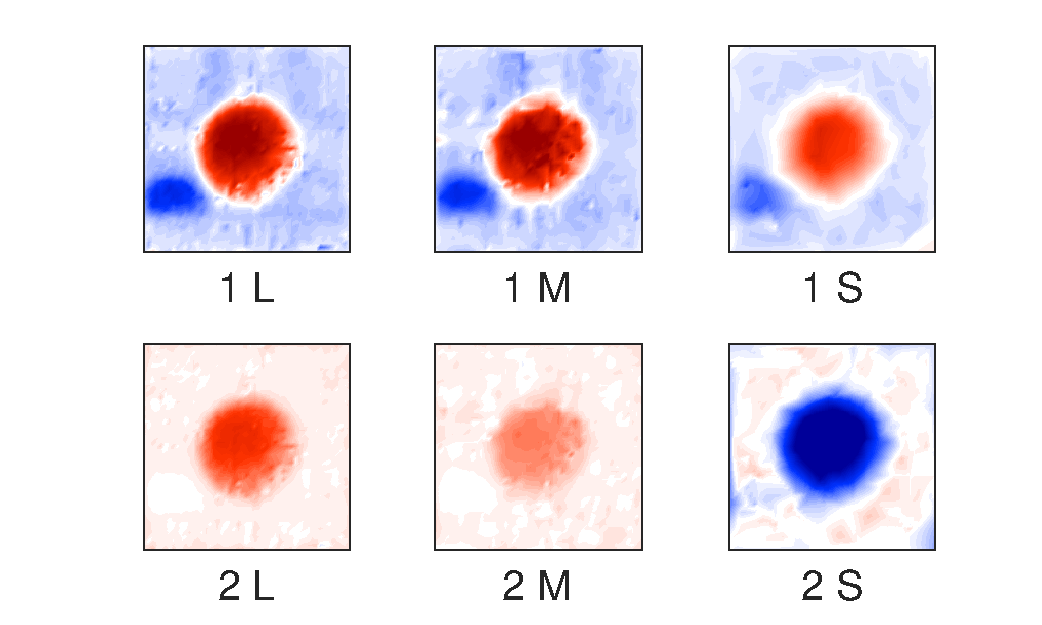
\includegraphics[width=\textwidth]{../Figures/Figure10/Figure10_a.pdf}
        \caption{RF response Case 2}
        \label{fig:case2RFResponse}
    \end{subfigure}
        \begin{subfigure}[b]{0.3 \textwidth}
        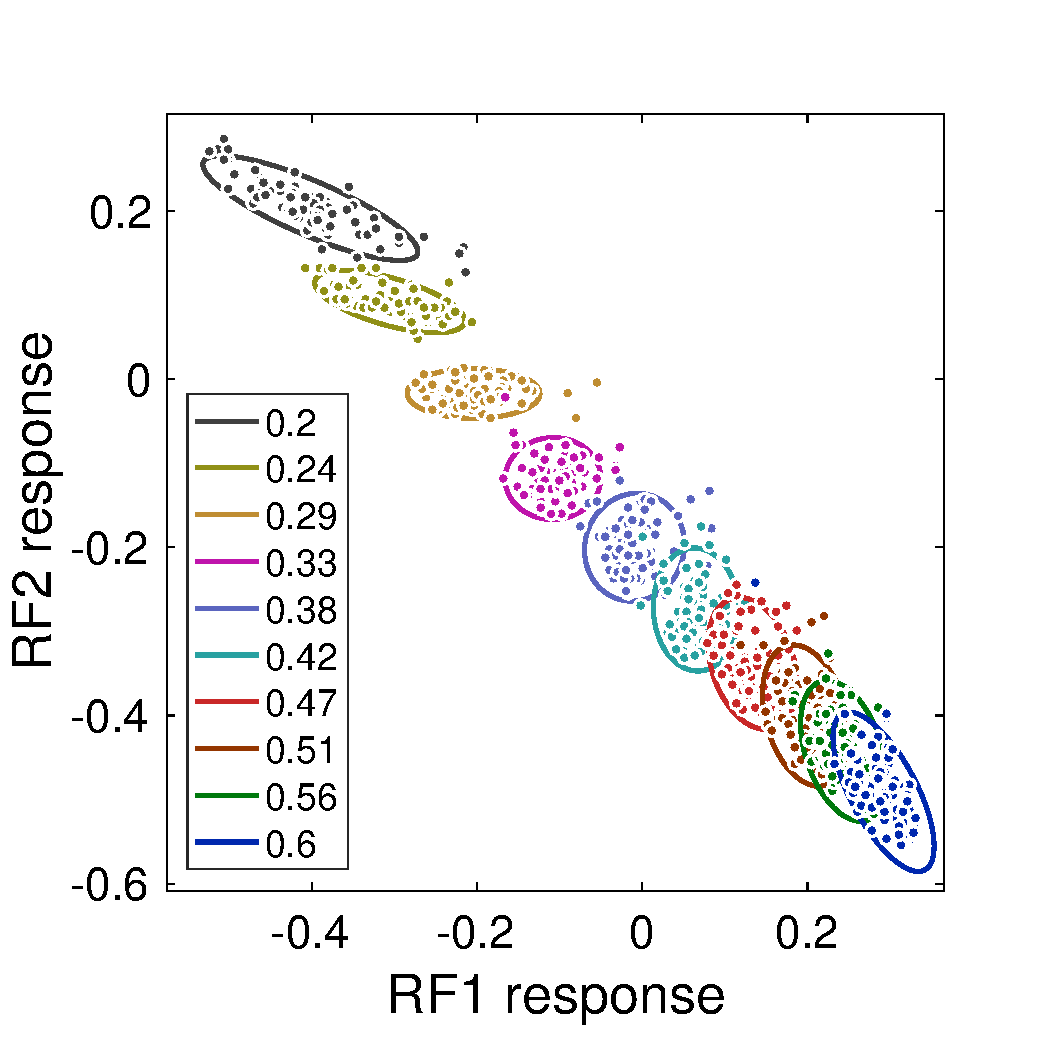
\includegraphics[width=\textwidth]{../Figures/Figure10/Figure10_b.pdf}
        \caption{Luminance Estimates}
        \label{fig:case2Estimates}
    \end{subfigure}
            \begin{subfigure}[b]{0.3 \textwidth}
        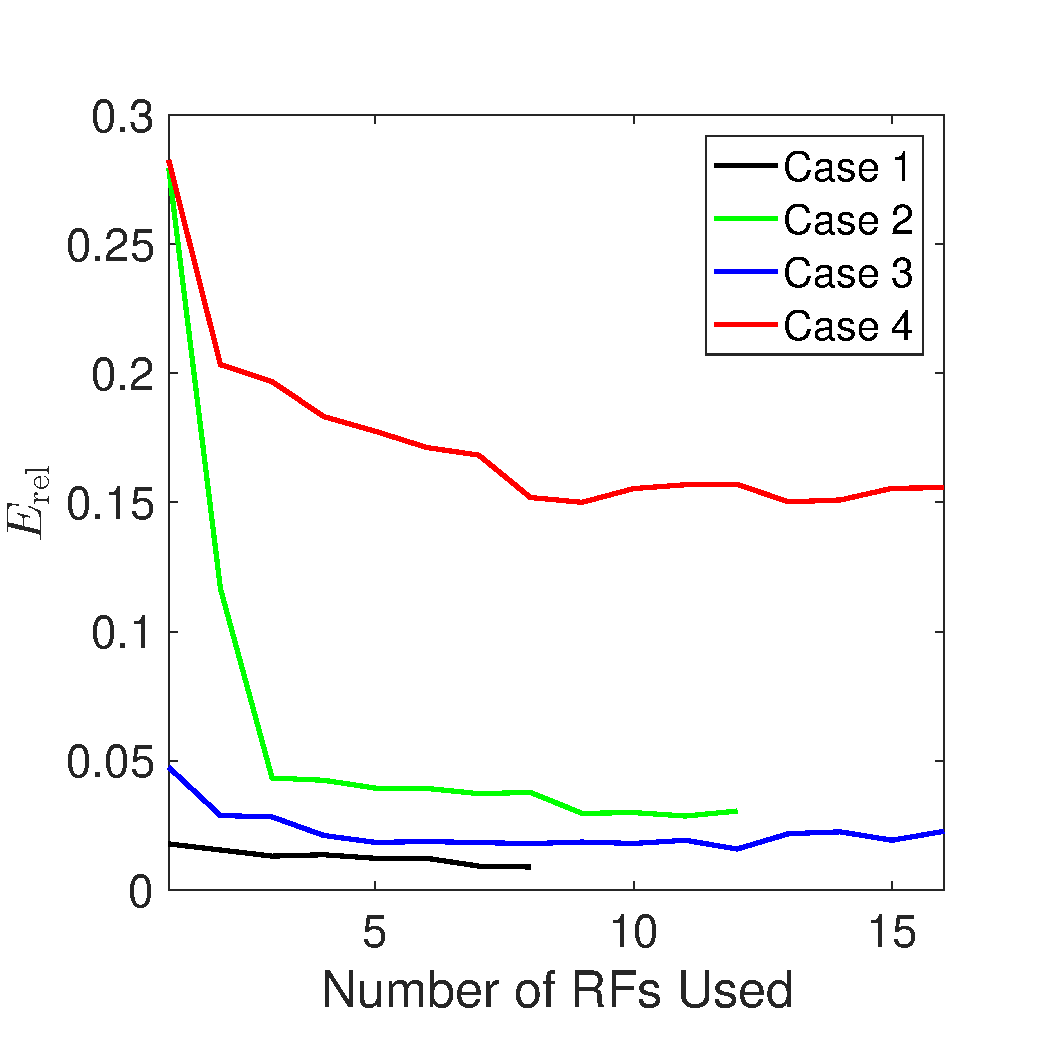
\includegraphics[width=\textwidth]{../Figures/Figure10/Figure10_c.pdf}
        \caption{Error v/s number of RFs}
        \label{fig:ErrorVsNFilters}
    \end{subfigure}
    \caption{{\bf Case 2:} (a) Photoreceptor response projected along the first two AMA receptive fields. (b) Estimated v/s assigned target object luminance for the image in case 2. Solid lines show the mean estimate, the filled region in light color  shows one standard deviation. (c) Relative error as a function of number of AMA receptive fields used for luminance estimation. The relative error reduces if more receptive fields are used for estimation.}
\label{fig:case2Results}
\end{figure}

It has previously been assumed that the surface reflectance spectra of the background objects have no direct effect on the light reflected by the target object \cite{BrainardWandellRetinex}. This would suggest that the response of the photoreceptors corresponding to the target object would only depend on the surface reflectance spectrum of the target object. But our results show that the effects of change in background object surface reflectances are significant. The secondary reflections from the target object, of the light coming indirectly after being reflected from the background objects, contribute to response of the photoreceptors corresponding to the target object.

\subsubsection{Case 3: Target object relative surface reflectance spectrum variable, light source spectra variable, background object spectra fixed}
For images of case 3, the AMA receptive fields learnt using the photoreceptor response does a very poor job in predicting the target object luminance (Fig.~\ref{fig:isomerizationFails}). 
This is because, since the illuminant spectra varies in this case, the photoreceptor response is not directly proportional to the target object surface anymore. 
But, since the background surfaces are fixed in this case, the ratio between the response of  photoreceptors corresponding to the target object and the background remains proportional to the target object luminance. 
This is because a change in illuminant spectra produces the same effect in both the target object and the background object. 
Thus, the AMA receptive fields learnt on the contrast normalized photoreceptor response (see Methods) can be used to predicts the target object luminance (Fig.~\ref{fig:constrastWorks}). 
Fig.~\ref{fig:case10Results} shows the estimated target object luminance v/s the assigned luminance for the images in case 2 obtained using the contrast normalized representation. 
AMA receptive fields provide excellent predictions of the target object luminance. 
The predictions are much better compared to that of a linear model that only considers the (contrast normalized) response of the photoreceptors corresponding to the center pixel of the target object.

%% Figure Isomerization Fails
\begin{figure}
\centering
    \begin{subfigure}[b]{0.3	 \textwidth}   
        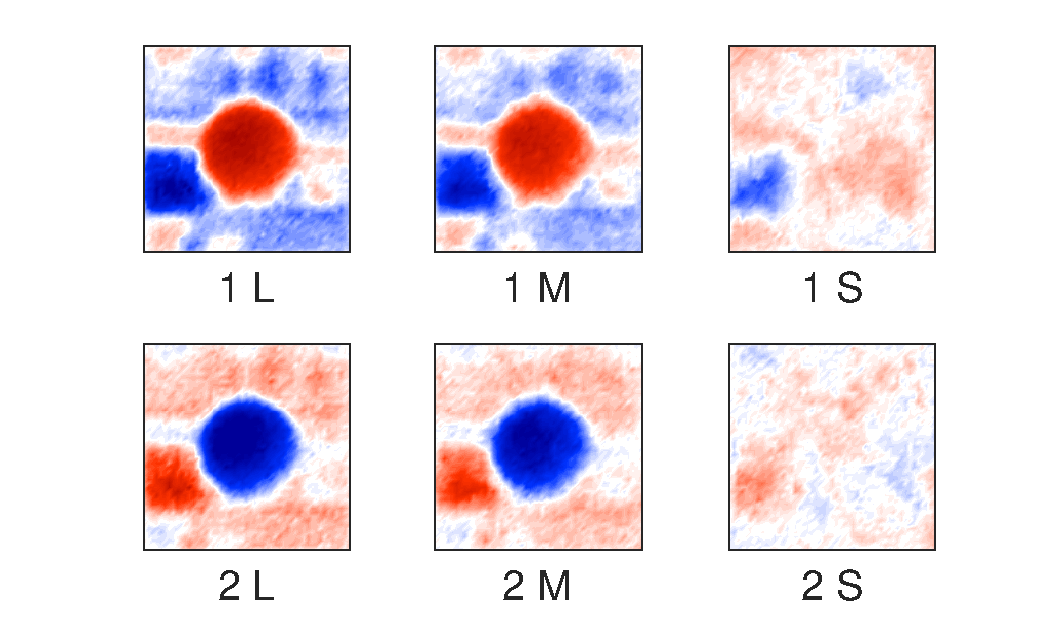
\includegraphics[width=\textwidth]{../Figures/Figure11/Figure11_a.pdf}
        \caption{RFs learnt using photoreceptor response}
        \label{fig:isomerizationFails}
    \end{subfigure}
        \begin{subfigure}[b]{0.3 \textwidth}
        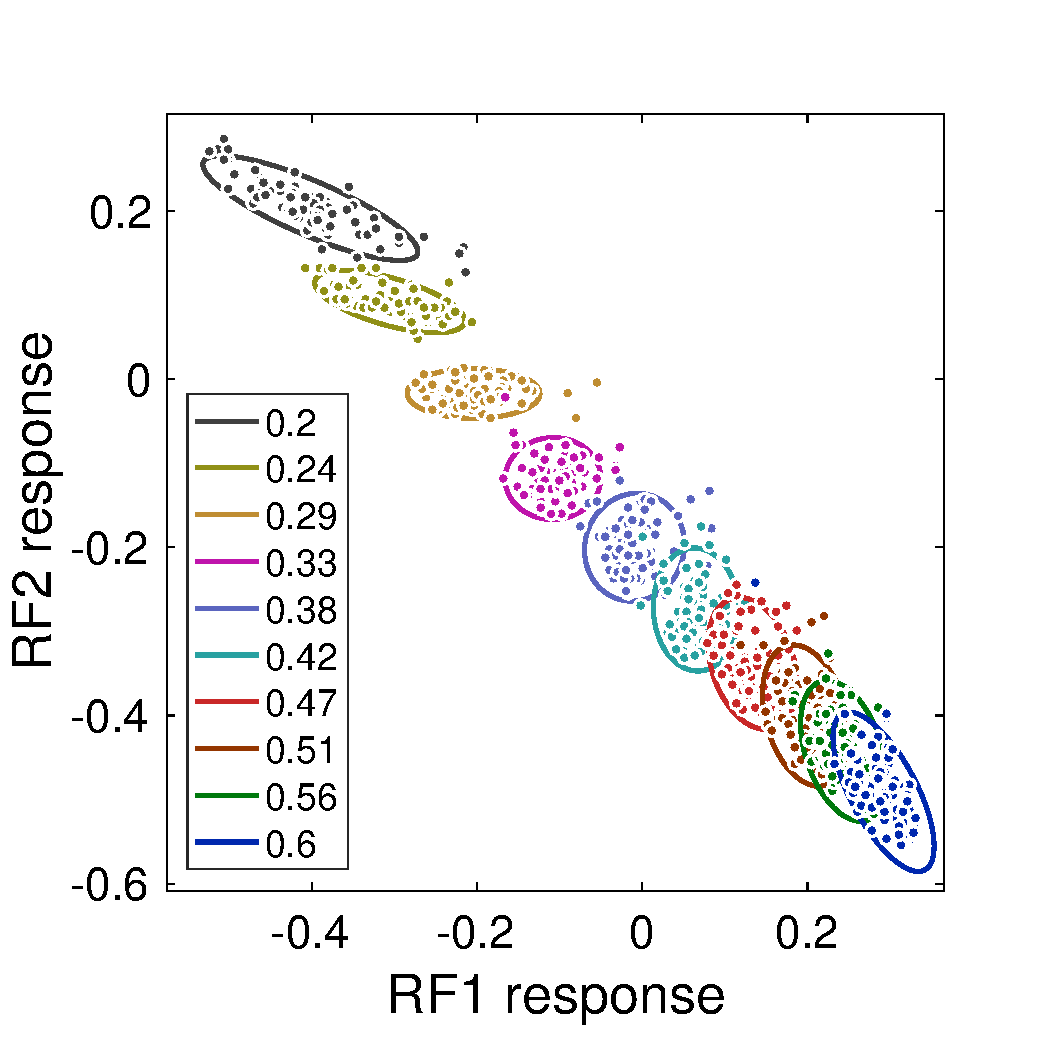
\includegraphics[width=\textwidth]{../Figures/Figure11/Figure11_b.pdf}
        \caption{RFs learnt using contrast signal}
        \label{fig:constrastWorks}
    \end{subfigure}
            \begin{subfigure}[b]{0.3 \textwidth}
        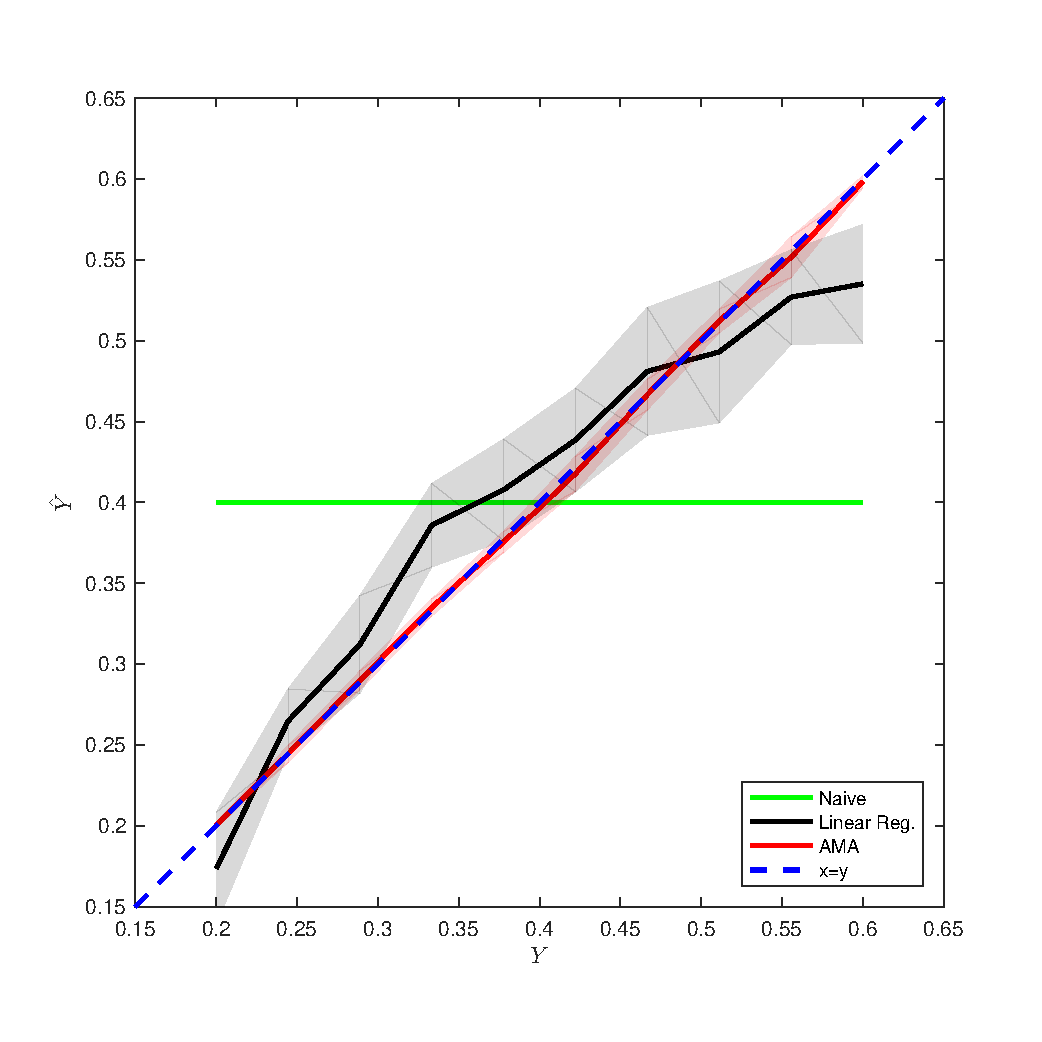
\includegraphics[width=\textwidth]{../Figures/Figure11/Figure11_c.pdf}
        \caption{Luminance estimates}
        \label{fig:case10Results}
    \end{subfigure}
    \caption{{\bf Case 2: Luminance can be estimated using the contrast signal:} (a) Photoreceptor response projected on AMA receptive fields calculated using photoreceptor response. (b) The contrast normalized photoreceptor response projected along the first two AMA receptive fields. The receptive fields were calculated using the contrast normalized stimuli. The response at each luminance level separates much better in this representation. (c) Estimated v/s assigned target object luminance for the image in case 2. Solid lines show the mean estimate, the filled region in light color  shows one standard deviation. AMA estimates are much better compared to the null models.}
\label{fig:importanceOfConstrast}
\end{figure}

Again, similar to case 2, the projection along the first two receptive fields shows an overlap between the stimuli at higher luminance values (Fig.~\ref{fig:constrastWorks}). But, the stimuli are better separated if the projection is considered within a subspace that has more receptive fields (Fig.~\ref{fig:ErrorVsNFilters}).

%%% Figure 11
%\begin{figure}
%\centering
%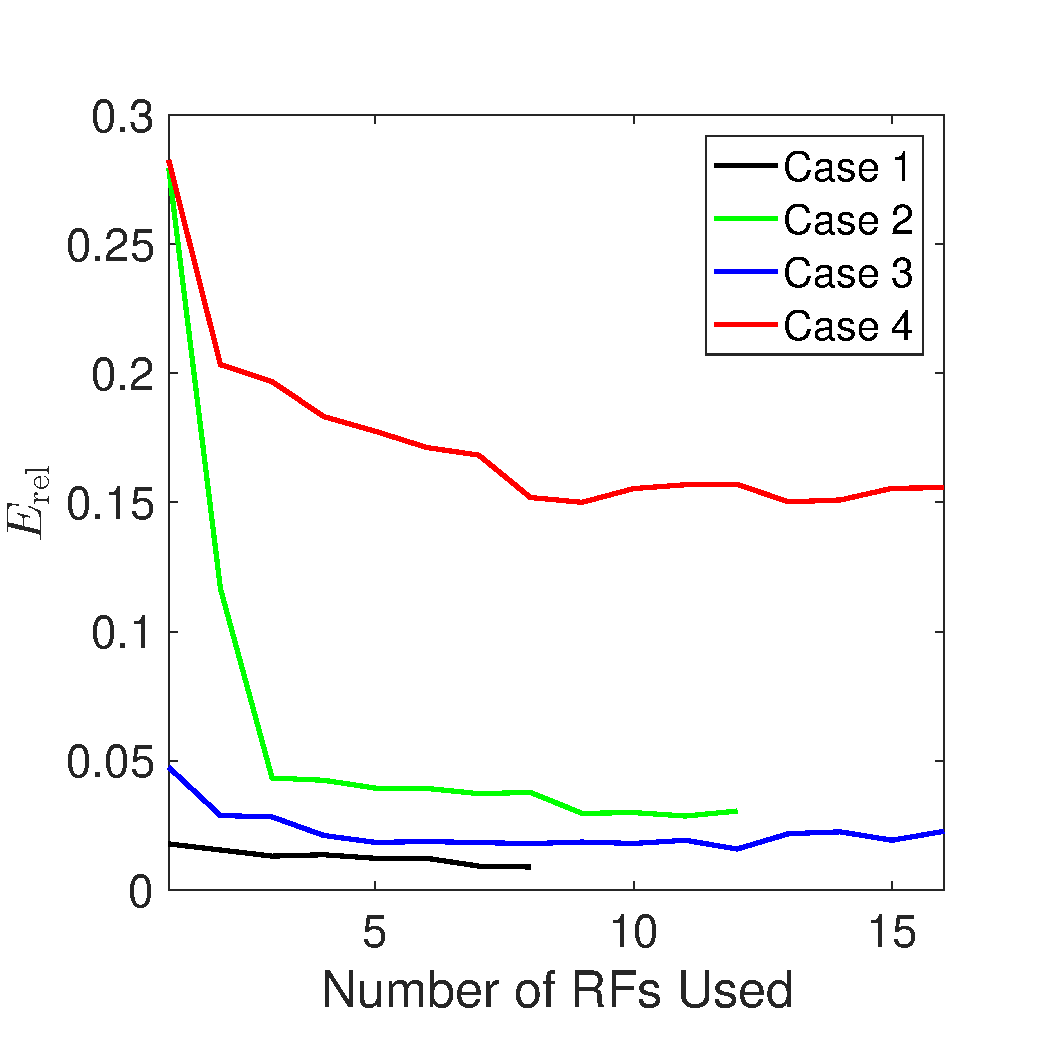
\includegraphics[width=0.3\textwidth]{../Figures/Figure11/Figure11.pdf}
%\caption{{\bf Performance with number of RFs used for estimation:} Most of the information is captured by the first two filters. We have used the first 8 RFs for estimating the luminance.}
%\label{fig:RMSEvsNFilters}
%\end{figure}
% GET RID OF AMA FROM THE CAPTION

\subsubsection{Case 4: Target object relative surface reflectance spectrum variable, light source spectra variable, background object spectra variable}
% Figure 12
\begin{figure}
\centering
    \begin{subfigure}[b]{0.3 \textwidth}   
        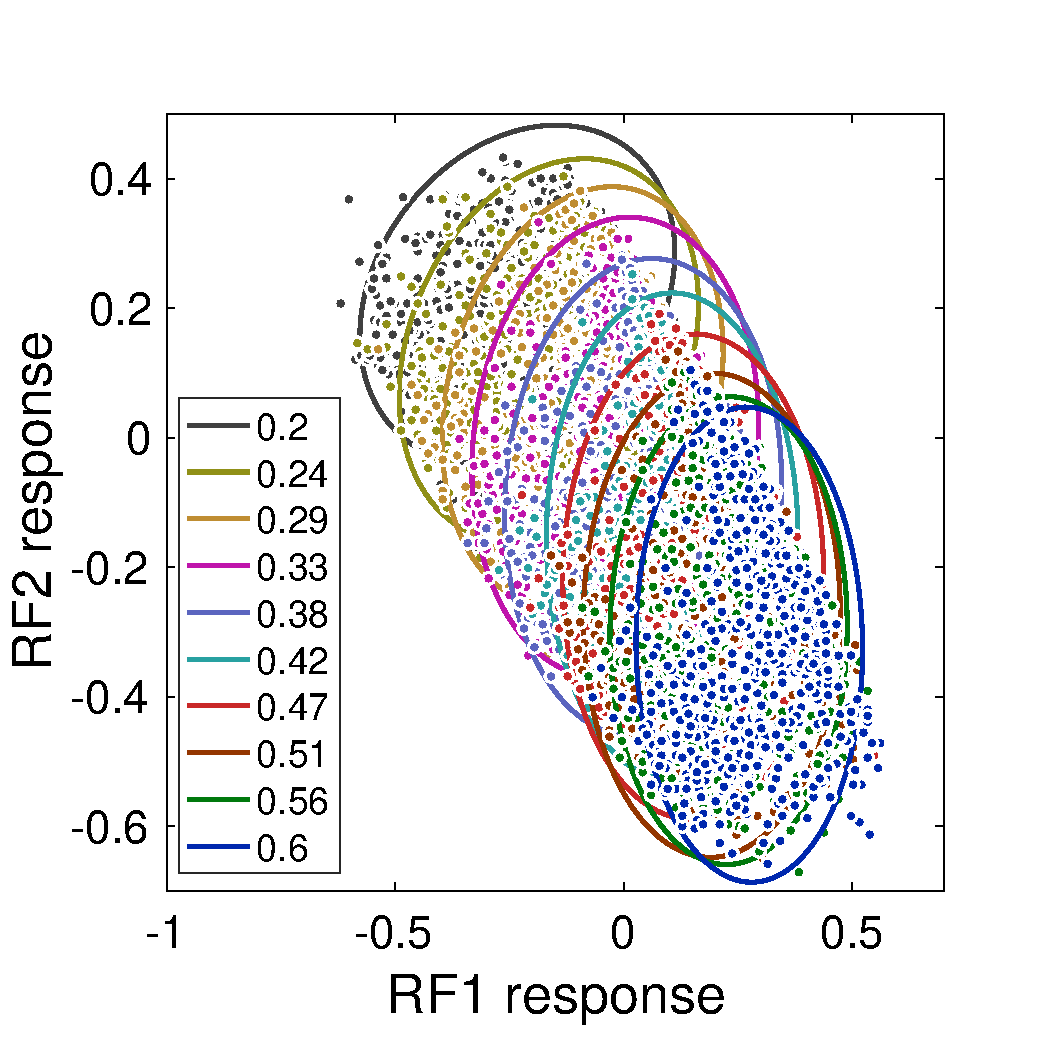
\includegraphics[width=\textwidth]{../Figures/Figure12/Figure12_a.pdf}
        \caption{AMA RF Response}
        \label{fig:case12FiltersResponse}
    \end{subfigure}    
        \begin{subfigure}[b]{0.3 \textwidth}
        \includegraphics[width=\textwidth]{../Figures/Figure12/Figure12_b.pdf}
        \caption{Luminance Estimates}
        \label{fig:case12Results}
    \end{subfigure}
    \caption{{\bf Case 3:} (a) Contrast normalized photoreceptor response projected along the first two AMA receptive fields. (b) Target object luminance estimates v/s assigned luminance for images in case 3. The AMA estimates are unbiased and have smaller relative error compared to linear model.}
    \label{fig:case12AllResults}
\end{figure}

Fig.~\ref{fig:case12AllResults} shows the AMA receptive field response and the luminance estimates for the images in case 3. 
We have used the first 8 receptive fields to estimate the luminance in this case (see Fig.\ref{fig:ErrorVsNFilters}). 
The AMA receptive fields do an excellent job of predicting the target object luminance. The estimates are unbiased with the mean estimates lying close the diagonal unit slope line (Fig.~\ref{fig:case12Results}). 
The relative error of estimation is $\sim15\%$, which low compared to that of the naive model ($\sim42\%$) or the linear model on center pixel ($\sim21\%$).

\subsection{Optimal receptive fields for luminance estimation have a center surround structure}
% Figure 14
\begin{figure}
\centering
\begin{subfigure}{0.21 \textwidth}
	\includegraphics[width=\textwidth]{../Figures/Figure13/Figure13_a.pdf}
	\caption{Case 1}
	\label{fig:case1Filter}
    \end{subfigure}
    ~ ~ ~
    \begin{subfigure}{0.21 \textwidth}   
	\includegraphics[width=\textwidth]{../Figures/Figure13/Figure13_b.pdf}
	\caption{Case 2}
	\label{fig:case2Filter}
    \end{subfigure}
    ~ ~ ~
        \begin{subfigure}{0.21 \textwidth}
	\includegraphics[width=\textwidth]{../Figures/Figure13/Figure13_c.pdf}
	\caption{Case 3}
	\label{fig:case3Filter}
    \end{subfigure}
    ~ ~ ~
        \begin{subfigure}{0.21 \textwidth}
	\includegraphics[width=\textwidth]{../Figures/Figure13/Figure13_d.pdf}
	\caption{Case 4}
	\label{fig:case4Filter}
    \end{subfigure}
\caption{{\bf AMA receptive fields:} The first two AMA receptive fields for the four cases studied in this work. The receptive fields show a center surround structure. The L and M filters have larger weight as luminance is essentially a function of the L and M cone isomerizations. The stereotypical pattern in the receptive fields of case 4 is due to the fixed geometry of the images.}
 \label{fig:AMAFilters}
\end{figure}

Fig.~{fig:AMAFilters} shows the first two AMA receptive fields that are optimal for luminance estimation for the spectral variations studied in this work. The receptive fields are ranked in ascending order of the value of the cost function associated with them. Thus the first RF corresponds to the direction along which the projection of the data gives the minimum cost. The L, M and S components give the weights for the linear sum of the cone responses for the three cone types. The salient features are: the center surround structure of the RFs and the higher weights of the L and M cones, compared to the S cones. 

For case 1, since the illuminant and the background are fixed, all the information is in the central target object reflectance. Thus, the RFs weights are mostly concentrated around the center. For case 2, where the target and the background spectra varies, most of the luminance information is still concentrated around the central target object. For case 3, while the target and the illuminant spectra varies, the background object spectra is fixed. Hence, the luminance can be estimated by simply from the contrast between the response of the cones corresponding to the target and the background. Thus, while the RFs show a trend of weights concentrated at the center similar to case 1, there is large negative contribution from the surround. The spatial features of the RFs are due the stereotypical geometry of the images (see \nameref{Methods}). Case 4 has a similar center surround structure, but with more prominent features of the background since the spectra of the background objects are also varying. Again, the spatial features are a result of the stereotypical geometry of the images.

\subsection{The receptive fields of complex case generalize on simpler cases}
Fig.~\ref{fig:barGraphs} shows the relative error for the estimates of the target object luminance obtained using the linear model and AMA. We show the relative error of the estimates obtained using the AMA receptive fields from all cases. The receptive fields from a more complex case perform at par on the stimuli from a simpler case. The optimal AMA estimates are better than that of the linear model.

% Figure 14
\begin{figure}
\centering
\begin{subfigure}{0.22 \textwidth}
	\includegraphics[width=\textwidth]{../Figures/Figure14/Figure14_a.pdf}
	\caption{Case 1}
	\label{fig:case1Bar}
    \end{subfigure}
    ~ 
    \begin{subfigure}{0.22 \textwidth}   
	\includegraphics[width=\textwidth]{../Figures/Figure14/Figure14_b.pdf}
	\caption{Case 2}
	\label{fig:case2Bar}
    \end{subfigure}
    ~ 
        \begin{subfigure}{0.22 \textwidth}
	\includegraphics[width=\textwidth]{../Figures/Figure14/Figure14_c.pdf}
	\caption{Case 3}
	\label{fig:case3Bar}
    \end{subfigure}
    ~ 
        \begin{subfigure}{0.22 \textwidth}
	\includegraphics[width=\textwidth]{../Figures/Figure14/Figure14_d.pdf}
	\caption{Case 4}
	\label{fig:case4Bar}
    \end{subfigure}
\caption{{\bf Error comparison across models:} Comparison of optimal AMA receptive fields from one case on the images of other cases. (a) Relative error of the estimates obtained using the linear model and AMA. The AMA receptive fields of case 1, 2 and 3 are used to estimate the target object luminance of the test images from case 1. The AMA receptive fields from all three cases perform well in this case. (b) Relative error for images of case 2. As expected, the error of the linear model on the center pixel is higher than AMA. AMA receptive fields from case 1 do worse than the receptive fields from case 2 and 3. (c) Relative error for images of case 3. The best predictions are from the receptive learnt using the images of case 3.}
 \label{fig:barGraphs}
\end{figure}

\section{Discussion} \label{Discussion}
In this paper, we studied luminance constancy using naturalistic images. We generated a dataset of multispectral images labeled by the reflectance of a target object in each image. These images were generated by a software pipeline developed for this work that we call Virtual world color constancy (VWCC). This software creates 3D scene descriptors based on programatic information provided by the user. Such information include the shape of the 3D rendering space, the shape, size, position and material properties of the objects and light sources in the scene, the location of the observer, etc. We assign these geometrical and spectral properties (the power spectrum of the light sources and the surface reflectance of the objects) using random sampling from available databases of naturally occurring objects, light sources and surface reflectances. Thus, we generate a large database of labeled hyper-spectral images, with naturalistic scene properties, but with the information about the surface reflectance and illumination at every pixel in the image. Such databases are near to be impossible to generate using other means as it is very hard to measure the surface reflectance of every object and the illumination at every point, even for well controlled scenes in a lab.

In this paper, as a first step towards understanding color constancy using supervised methods on labeled dataset, we studied a simpler analogue: luminance constancy. We generated images labeled with the luminance of a target object in the scene. We performed three types of spectral manipulations in the scene while generating the images (Fig.~\ref{fig:studiedCases}). 1. Allow variations in the spectral shape of the target object surface reflectance spectrum, while keeping the background object surface reflectance and the illumination spectra of the light sources fixed. 2. Allow variations in the shape of the target object surface reflectance and the illumination spectra of the light sources, while keeping the surface reflectance spectra of the background objects fixed. 3. Allow variations in all three types of spectra. We generated hundreds of images at multiple luminance level of the target object for each of these three cases. Then using a model of the early visual system, we generated the response of the cones in the retina for each image in our database. These model retinal responses, along with the luminance label of the images, are then used as the input to supervised learning algorithms. Using our supervised methods, we leant that the target object luminance can be obtained from simple manipulation of the cone response for case where the spectral manipulations are restricted to at most two of the three possible sources of manipulations: the target object surface reflectance, the background object surface reflectances, the light source illumination spectra. In these cases, the luminance can be obtained by comparing the response of the cones corresponding to the target and the background objects. When all these three types of spectral variations are allowed simultaneously, one needs additional information to obtain the luminance of the target object. 

\bibliography{references}
\bibliographystyle{jovcite}

\end{document}

